\section{Number of Iterations}
\label{sec:num_iterations}

This appendix contains details from a study showing the performance of the unfolding method as a function of the number of iterations used. UniFold, with 10 iterations, was applied in 30 independent trials for three input variables of interest corresponding to the leading jet: 

\begin{itemize}
\item Leading jet number of charged tracks (\texttt{Ntracks\_trackj1})
\item Leading jet $p_T$ (\texttt{pT\_trackj1})
\item Leading jet $\tau_1$ (\texttt{tau1\_trackj1})
\end{itemize}

Each independent trial used Pythia MC16e as the Monte Carlo sample and Sherpa MC16e as the ``data'' sample. To calculate the statistical uncertainty at each iteration, Poisson bootstrapping was applied to approximate sampling with replacement for the Sherpa (i.e. ``data'') sample. This consisted of an event-by-event weight scaling for both reco- and truth-level Sherpa MC by a value sampled from a Poisson distribution $\texttt{Pois}(\lambda = w)$, where $w$ is the event weight. If a given event's weight is negative, the weight is instead scaled by $-\texttt{Pois}(\lambda = |w|)$.

The performance metrics measured as a function of iteration are: 
\begin{itemize}
\item $\chi^2$ Histogram Distance: $$d(x,y) = \frac{1}{2}\sum_i\frac{(x_i - y_i)^2}{(x_i + y_i)}$$
\item Relative Statistical Uncertainty ($\frac{\sigma}{N}$), where $\sigma$ represents the standard deviation of the weighted unfolded histograms per iteration across all trials, averaged across all bins, and $N$ represents the unfolded histogram weighted bin counts per iteration, averaged across all trials and bins. 
\item Average Trajectory of Final Bin, i.e. the ratio of the final bin of the unfolded histogram at each iteration to the target value at each iteration, at both the reco- and truth-level. As this bin has very low statistics, it's difficult to observe any meaningful change in its performance looking at the histograms alone. However, it's clear from looking at ratio plots at each iteration that the tails of the histogram distribution are the most affected by the inclusion of additional iterations. These plots summarize this average movement across multiple iterations.
\end{itemize}

In all plots in this section, ``Iteration 0'' corresponds to the Pythia and Sherpa distributions before any unfolding or bootstrapping is applied. As expected, the histogram distance $d(x,y)$ between these two distributions is largest before unfolding is applied, but the statistical uncertainty is exactly zero. 

In each of the following subsections for each of the three variables considered, we show the unfolded histogram ratios at each iteration for one of the independent trials, for illustration purposes, and then each of the three performance metrics detailed above. In each instance, histogram distance $d(x,y)$ quickly achieves good performance within 2-3 iterations and remains fairly stable. The relative statistical uncertainty also remains fairly constant at a value of approximately 1.25-1.5\% across each iteration. However, we do see some motivation to use more than 3 iterations due to the average trajectories of the final histogram bins, which tend to achieve good performance around 5 iterations. We therefore use 5 iterations for the default unfolding procedure.

\subsection{Leading jet number of charged tracks} 
\subsubsection{Ratios of unfolded histograms for one trial}
\begin{figure}[]
\centering
\subfloat[Iteration 0 (before unfolding/bootstrapping)]{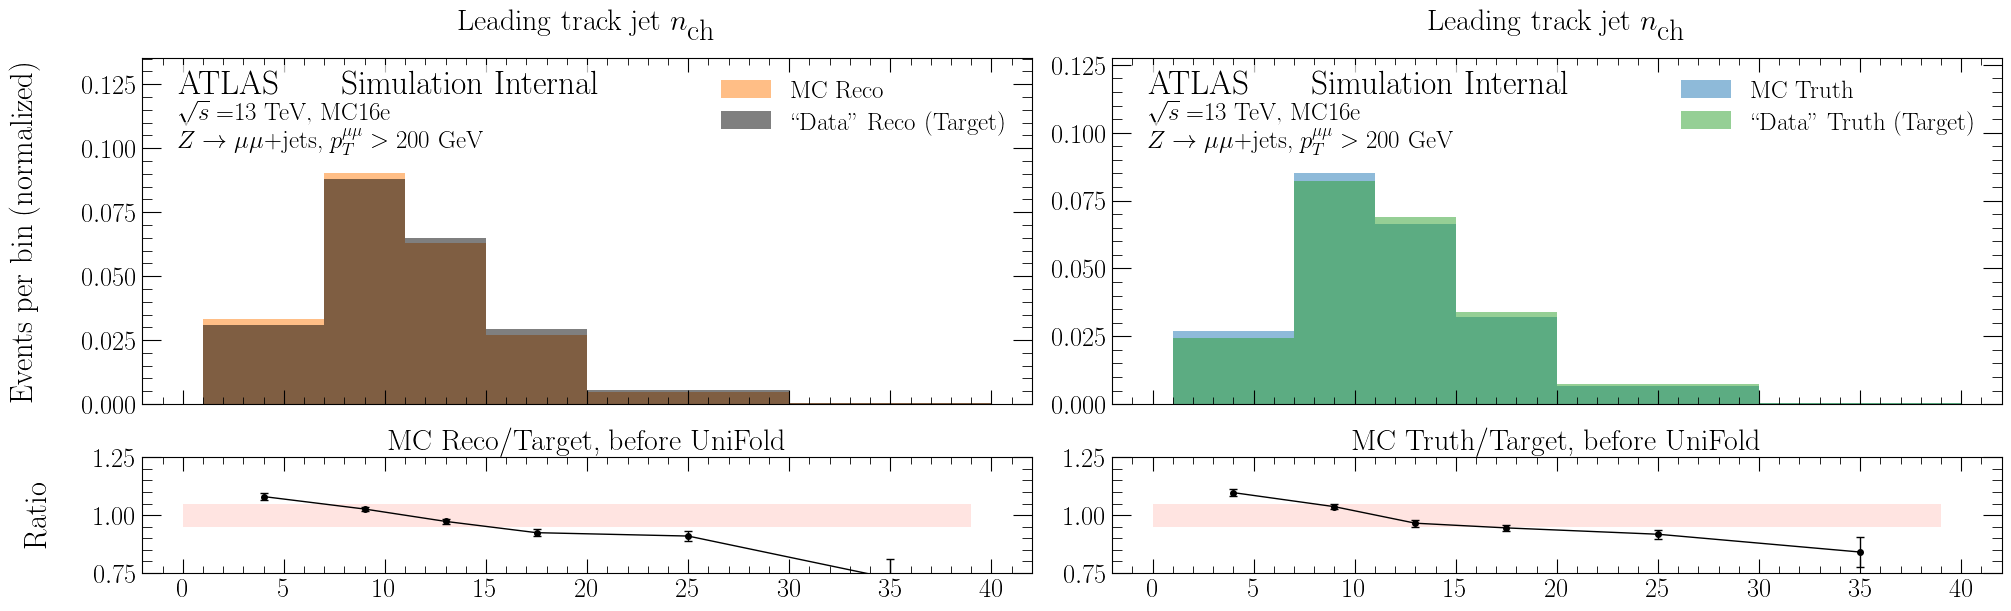
\includegraphics[width=0.95\textwidth]{figures/num_iterations_study/Ntracks_trackj1/iteration_study_30x10-Iteration00.png}}\\
\subfloat[Iteration 1]{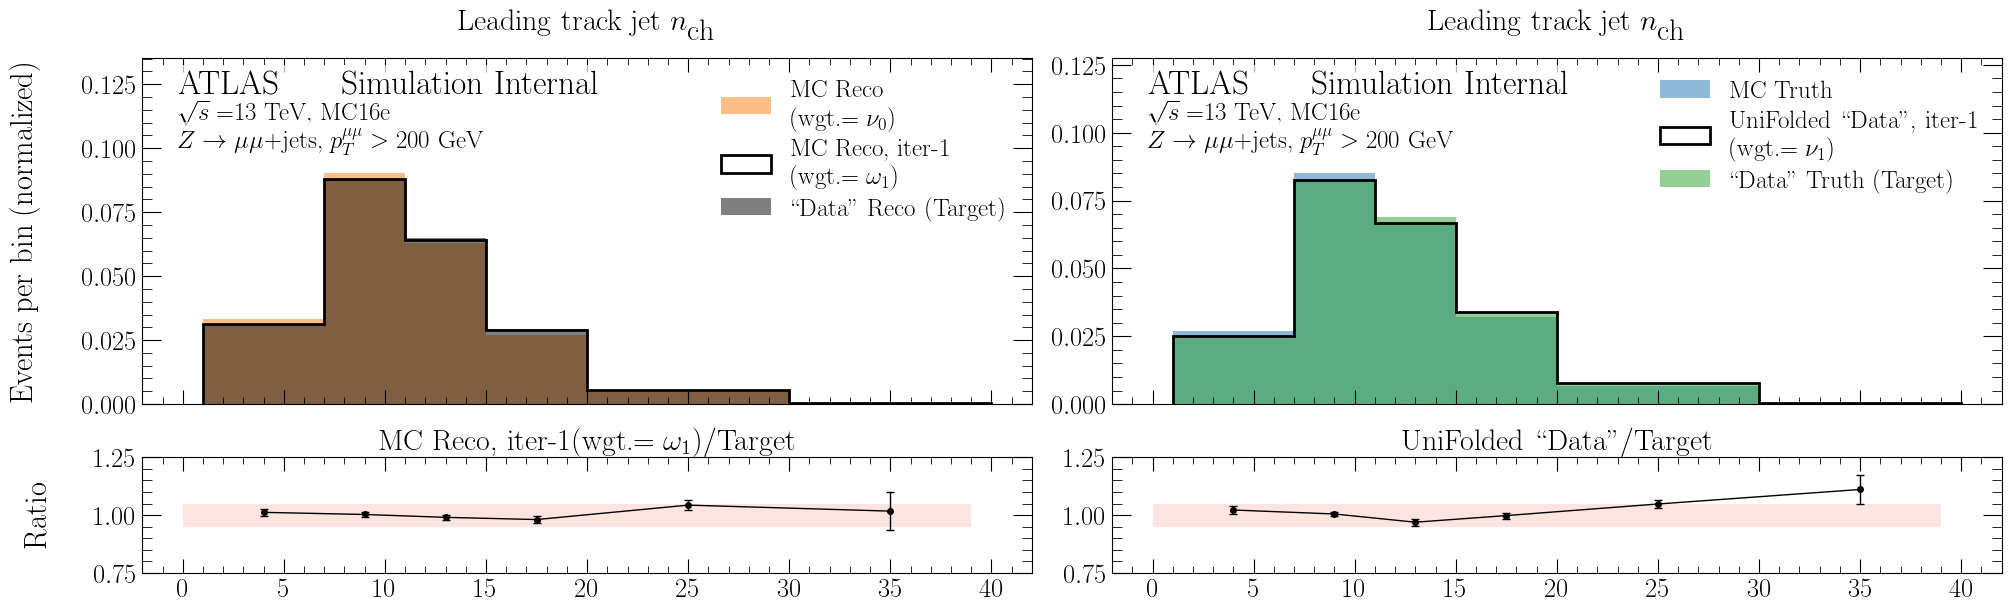
\includegraphics[width=0.95\textwidth]{figures/num_iterations_study/Ntracks_trackj1/iteration_study_30x10-Iteration01.png}}\\
\subfloat[Iteration 2]{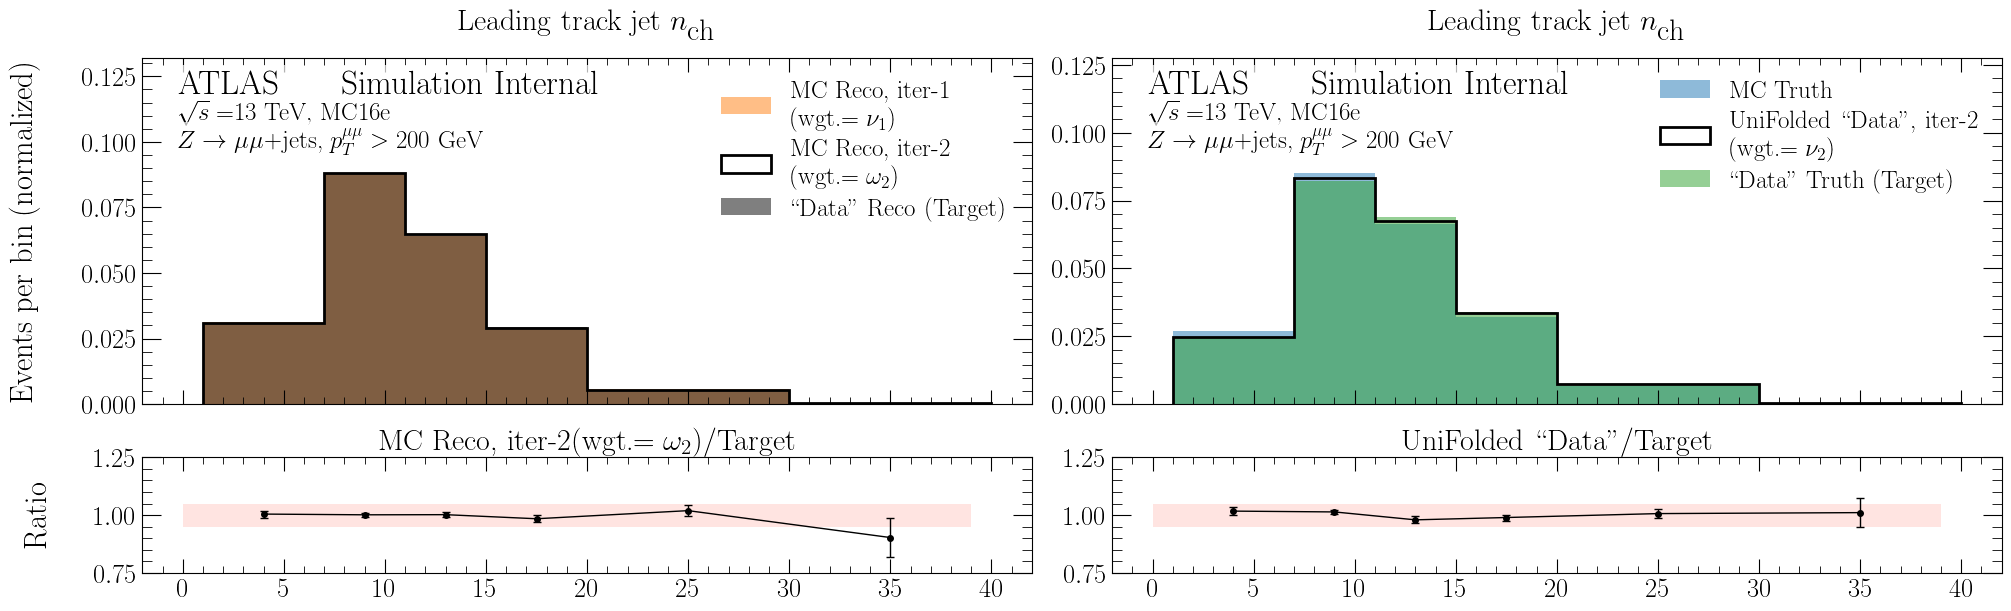
\includegraphics[width=0.95\textwidth]{figures/num_iterations_study/Ntracks_trackj1/iteration_study_30x10-Iteration02.png}}\\
\subfloat[Iteration 3]{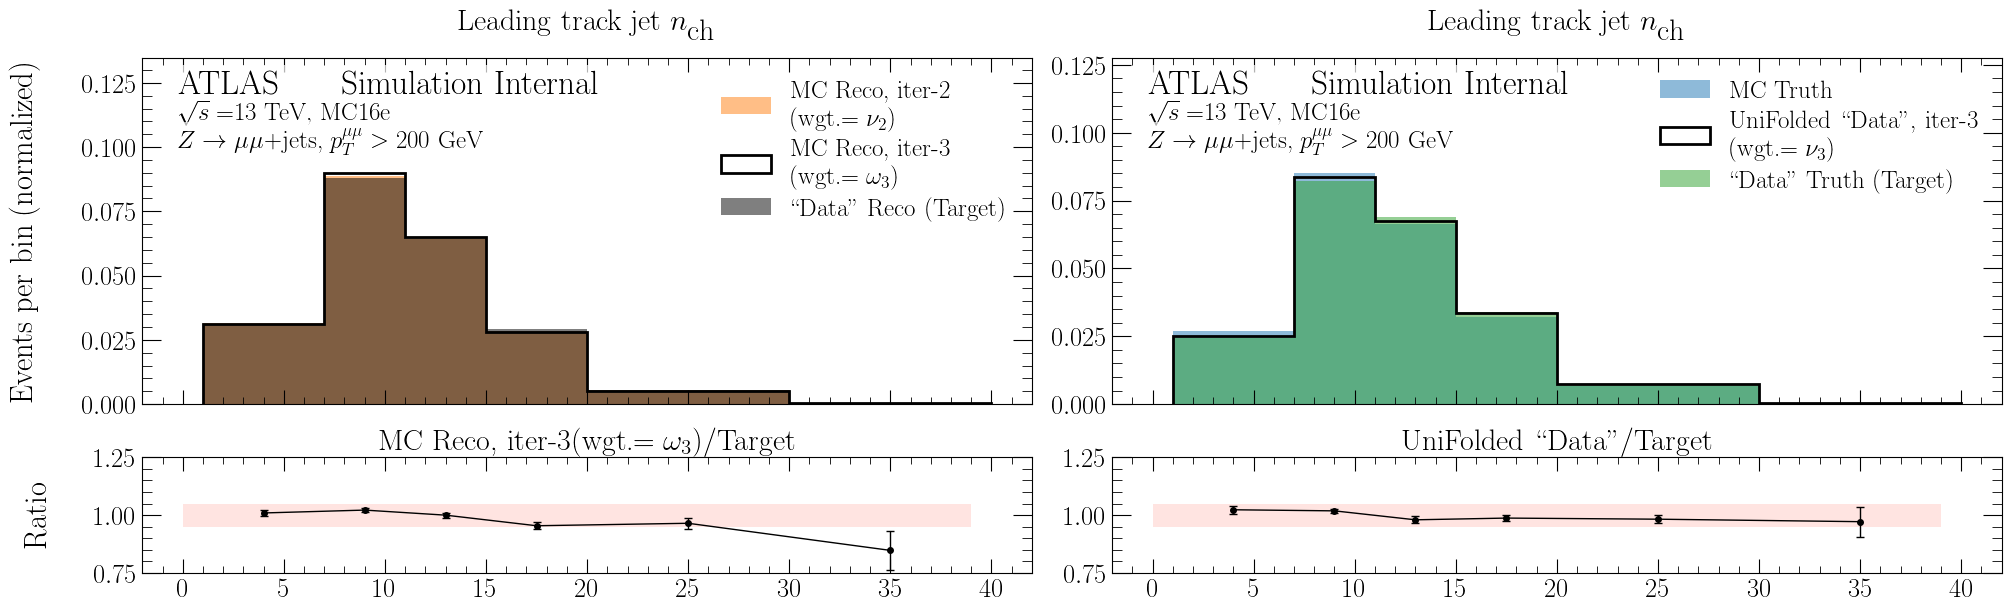
\includegraphics[width=0.95\textwidth]{figures/num_iterations_study/Ntracks_trackj1/iteration_study_30x10-Iteration03.png}}
\phantomcaption
\end{figure}
\begin{figure}[]
\centering
\ContinuedFloat
\subfloat[Iteration 4]{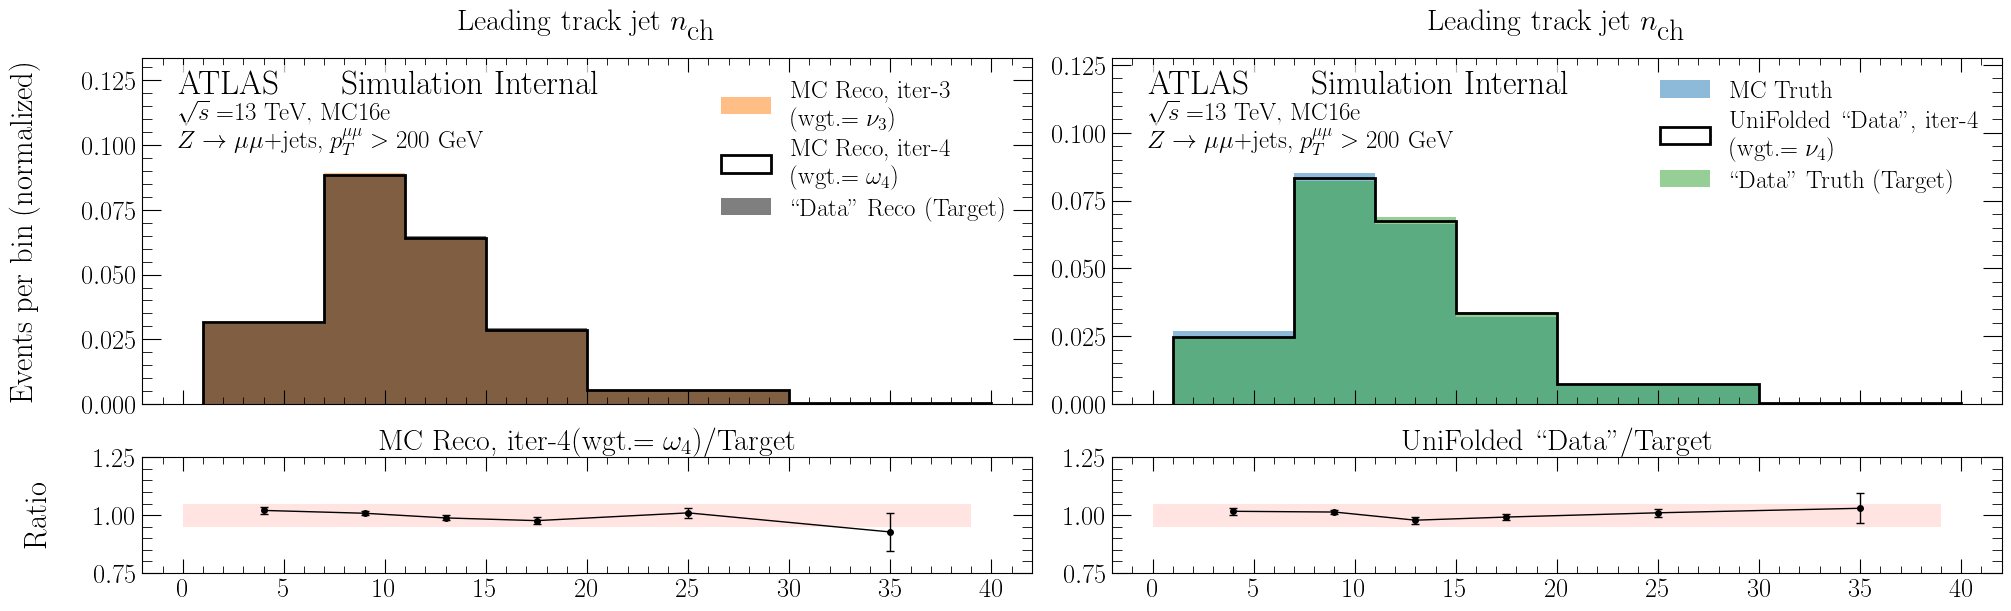
\includegraphics[width=0.95\textwidth]{figures/num_iterations_study/Ntracks_trackj1/iteration_study_30x10-Iteration04.png}}\\
\subfloat[Iteration 5]{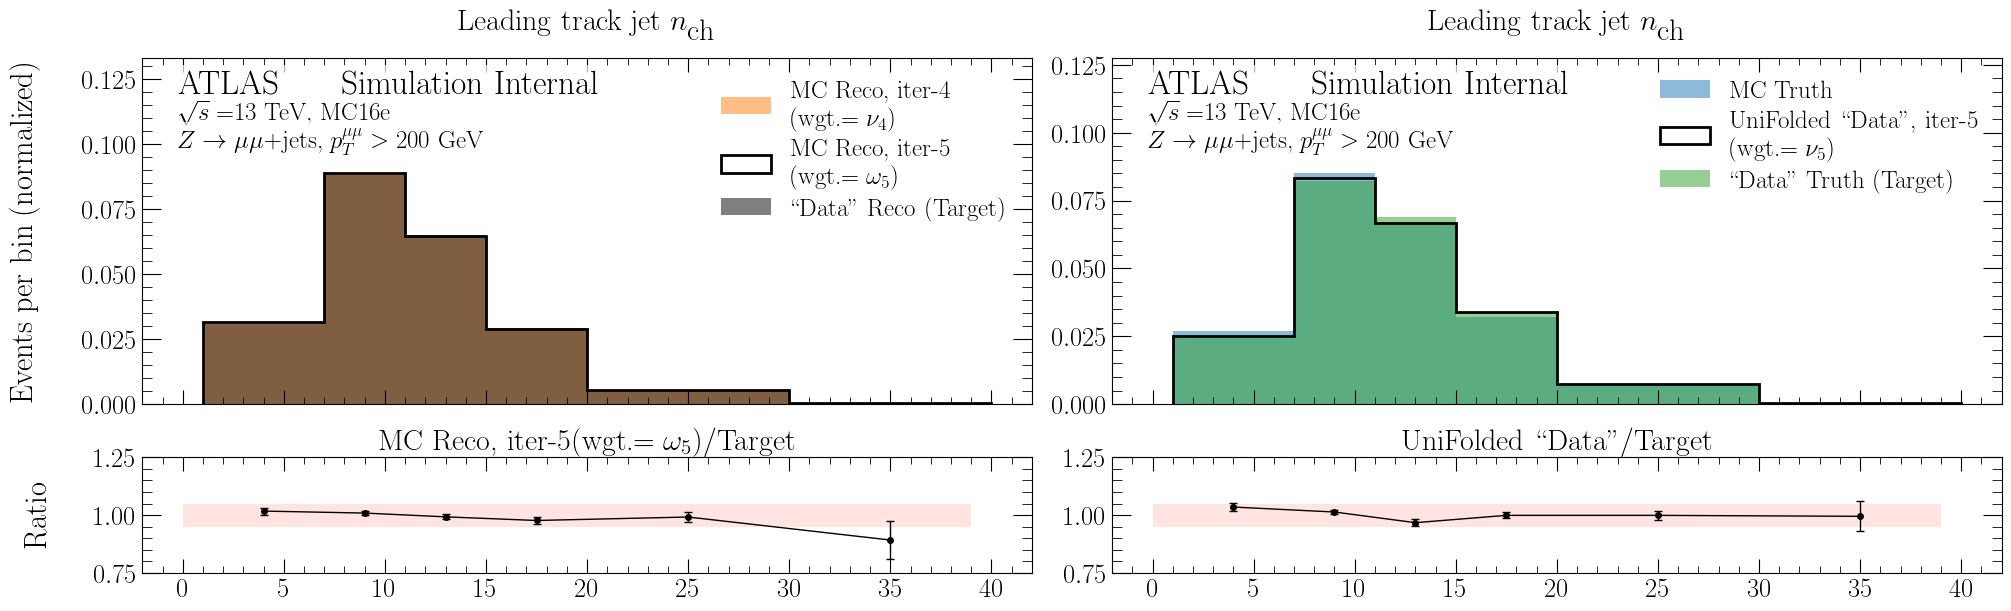
\includegraphics[width=0.95\textwidth]{figures/num_iterations_study/Ntracks_trackj1/iteration_study_30x10-Iteration05.png}}\\
\subfloat[Iteration 6]{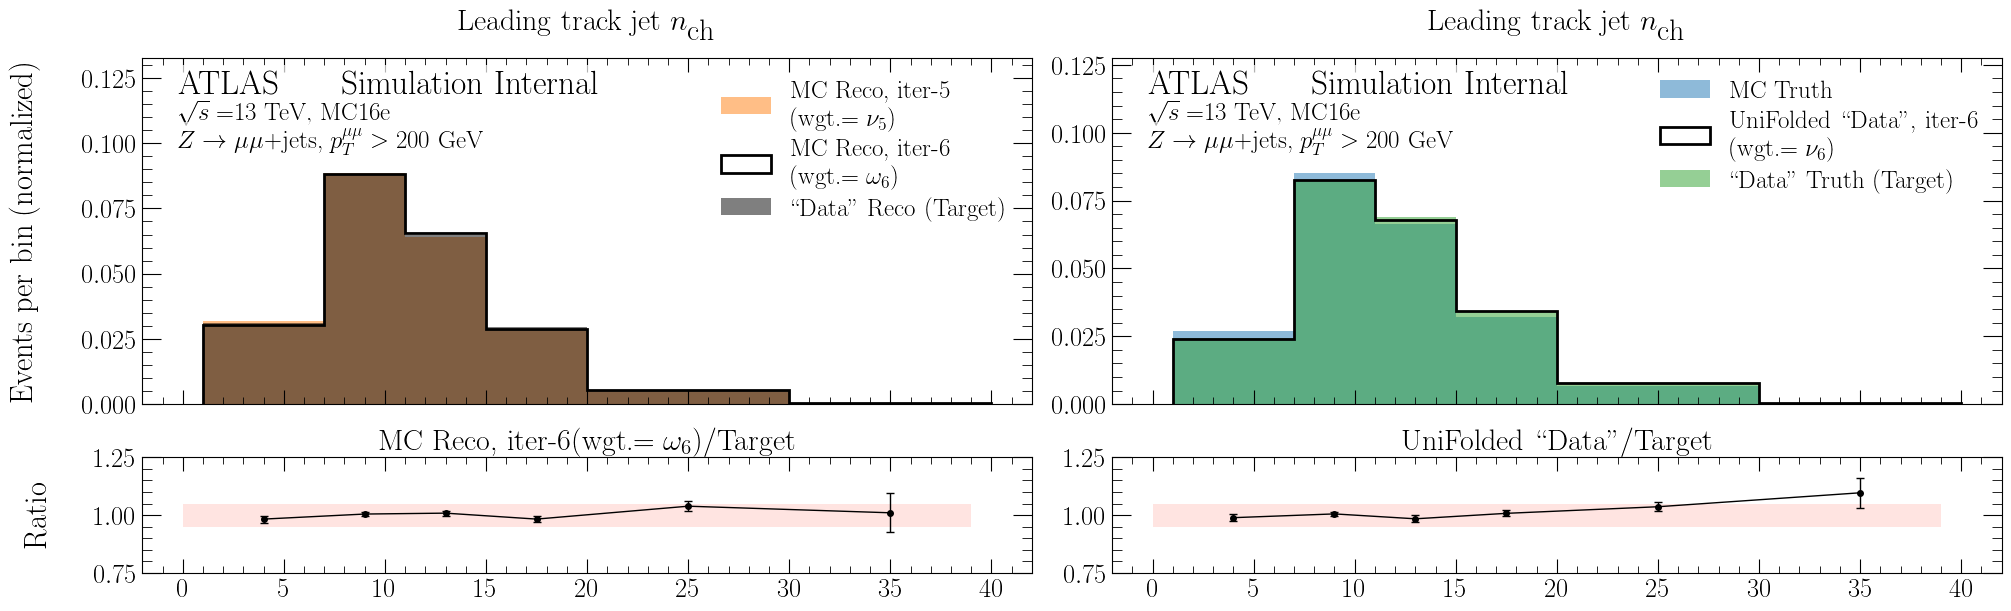
\includegraphics[width=0.95\textwidth]{figures/num_iterations_study/Ntracks_trackj1/iteration_study_30x10-Iteration06.png}}\\
\subfloat[Iteration 7]{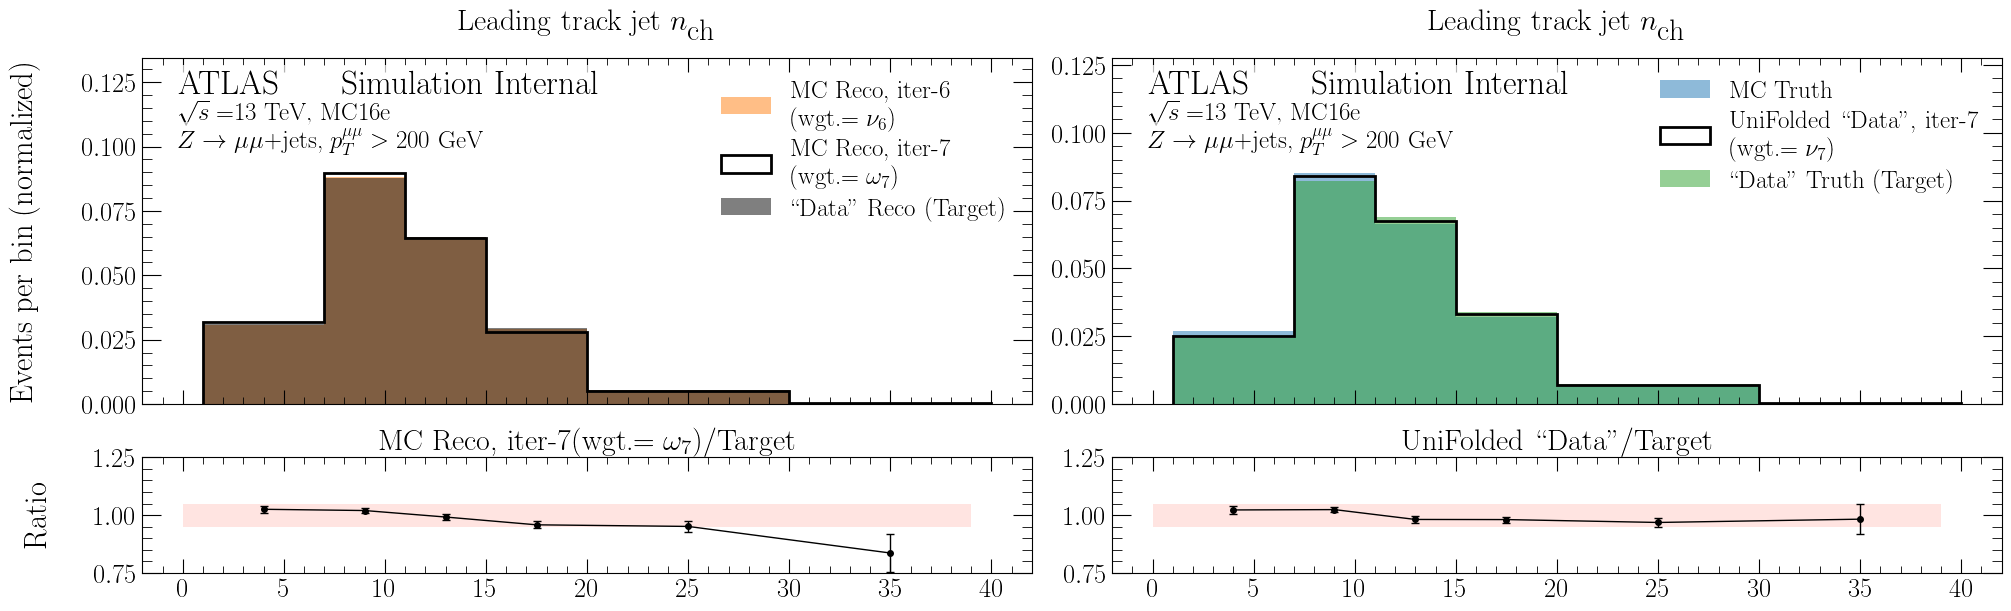
\includegraphics[width=0.95\textwidth]{figures/num_iterations_study/Ntracks_trackj1/iteration_study_30x10-Iteration07.png}}
\phantomcaption
\end{figure}
\begin{figure}[]
\centering
\ContinuedFloat
\subfloat[Iteration 8]{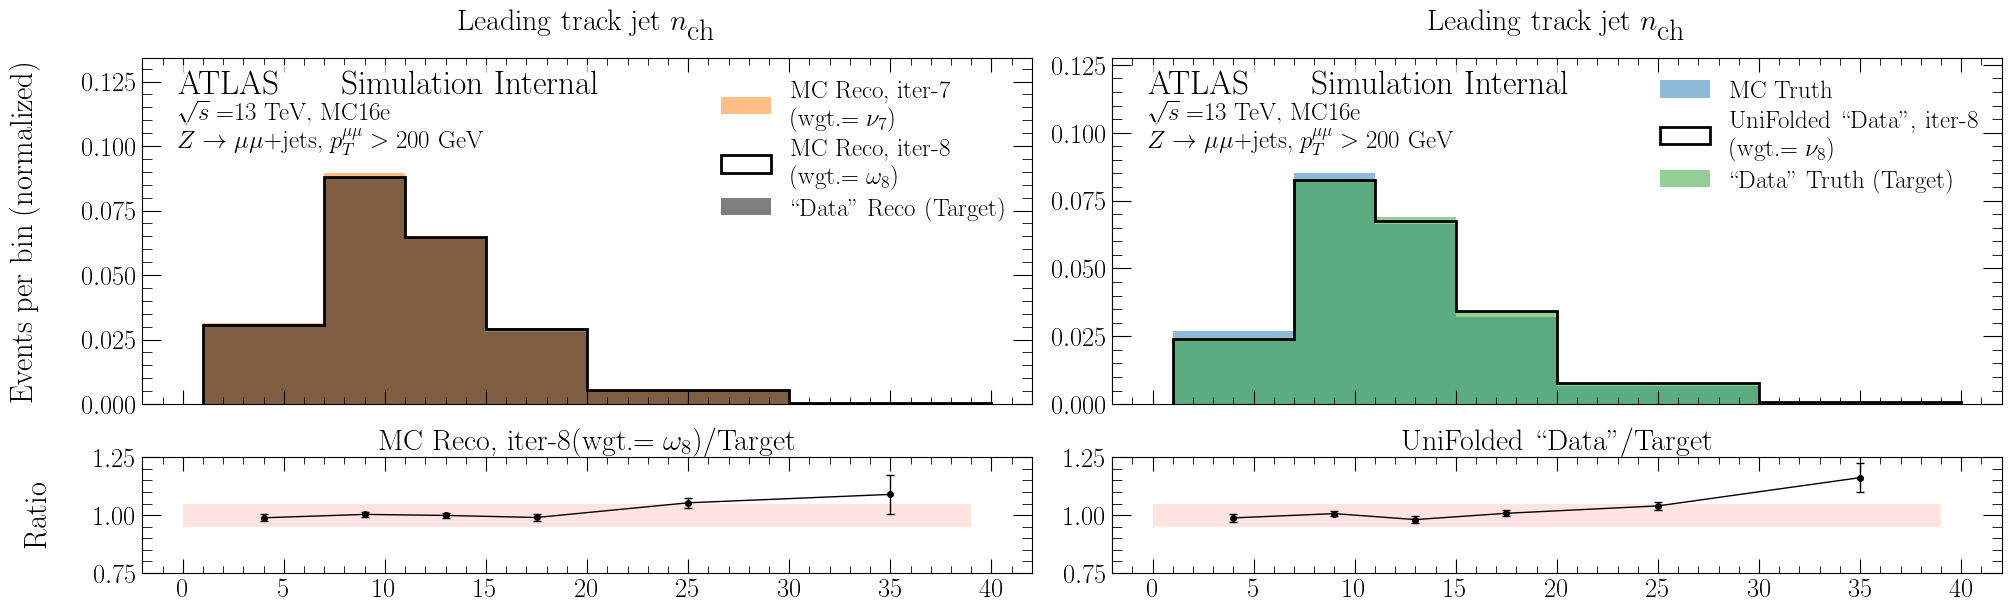
\includegraphics[width=0.95\textwidth]{figures/num_iterations_study/Ntracks_trackj1/iteration_study_30x10-Iteration08.png}}\\
\subfloat[Iteration 9]{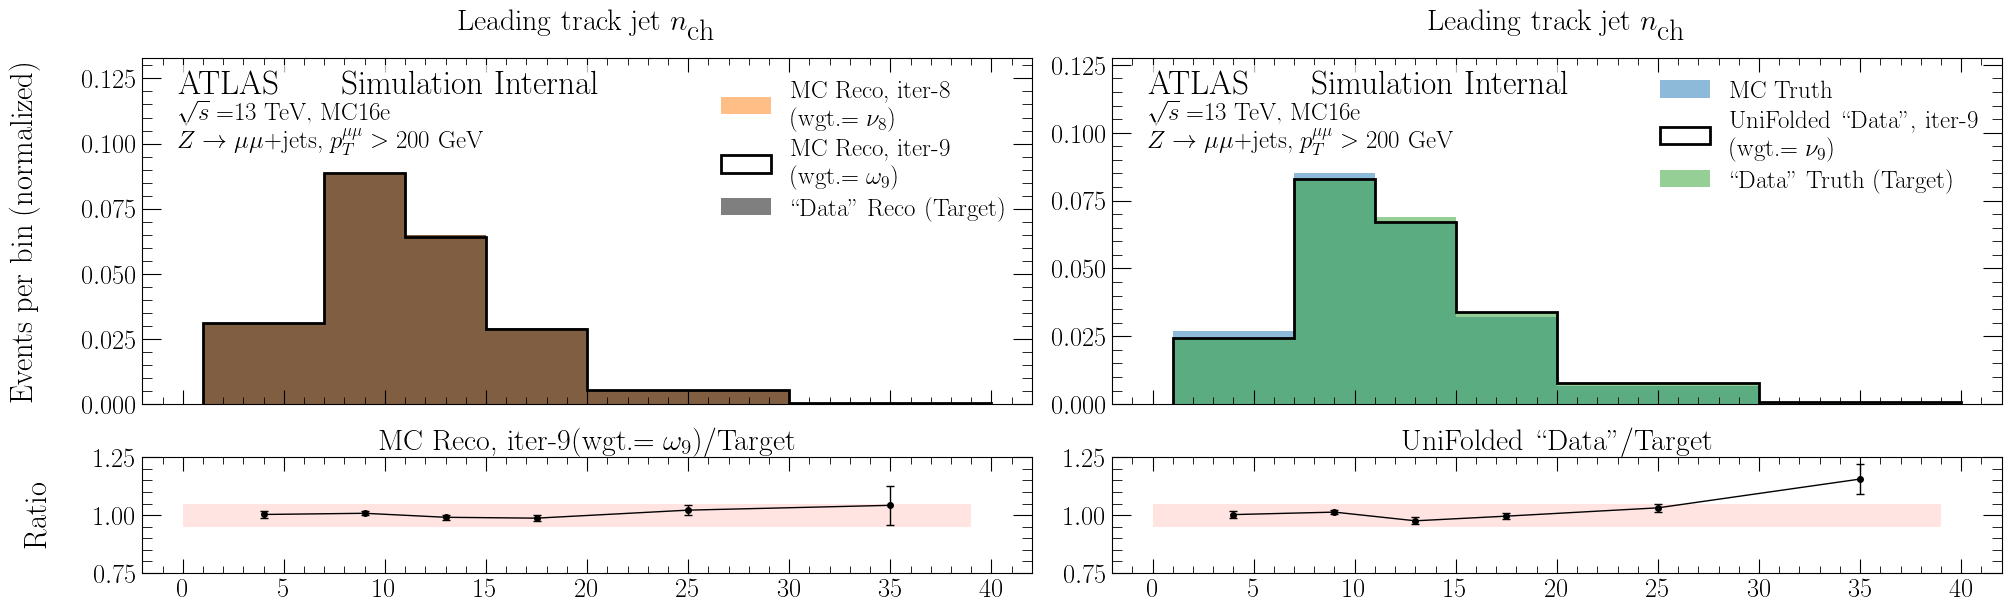
\includegraphics[width=0.95\textwidth]{figures/num_iterations_study/Ntracks_trackj1/iteration_study_30x10-Iteration09.png}}\\
\subfloat[Iteration 10]{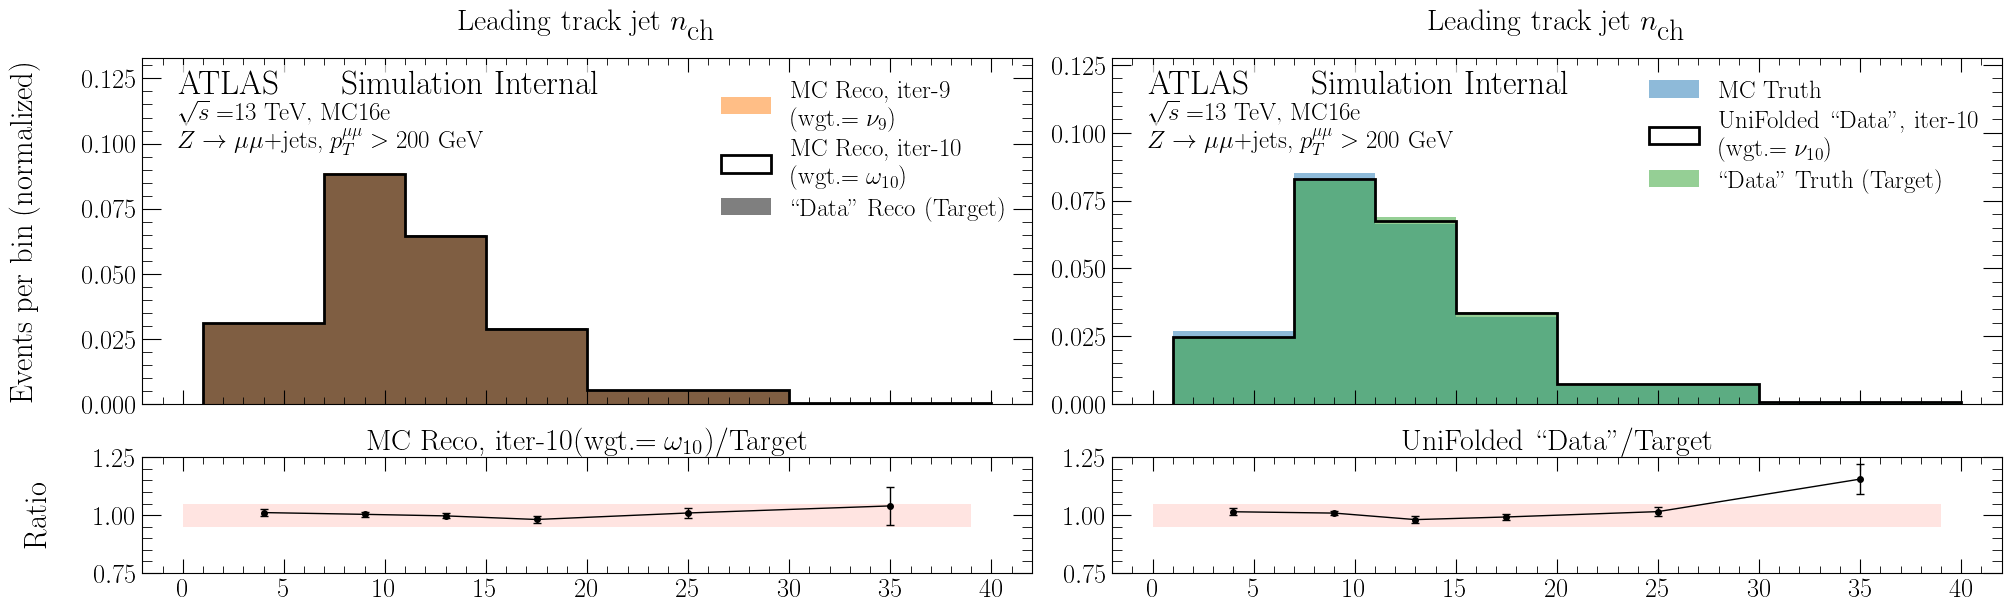
\includegraphics[width=0.95\textwidth]{figures/num_iterations_study/Ntracks_trackj1/iteration_study_30x10-Iteration10.png}}
\caption{\textbf{Leading jet $n_{\text{charged tracks}}$:} The unfolded histograms for UniFold in a single trial with Poisson bootstrapping applied. The ratio plots reveal that the bulk of the distribution quickly achieves good performance after about two iterations, but the tails of the distribution can sometimes benefit from additional iterations.}
\label{fig:num_iterations:ntracks_ratios}
\end{figure}


\subsubsection{Performance as a function of iteration}
\begin{figure}[!htb]
\centering
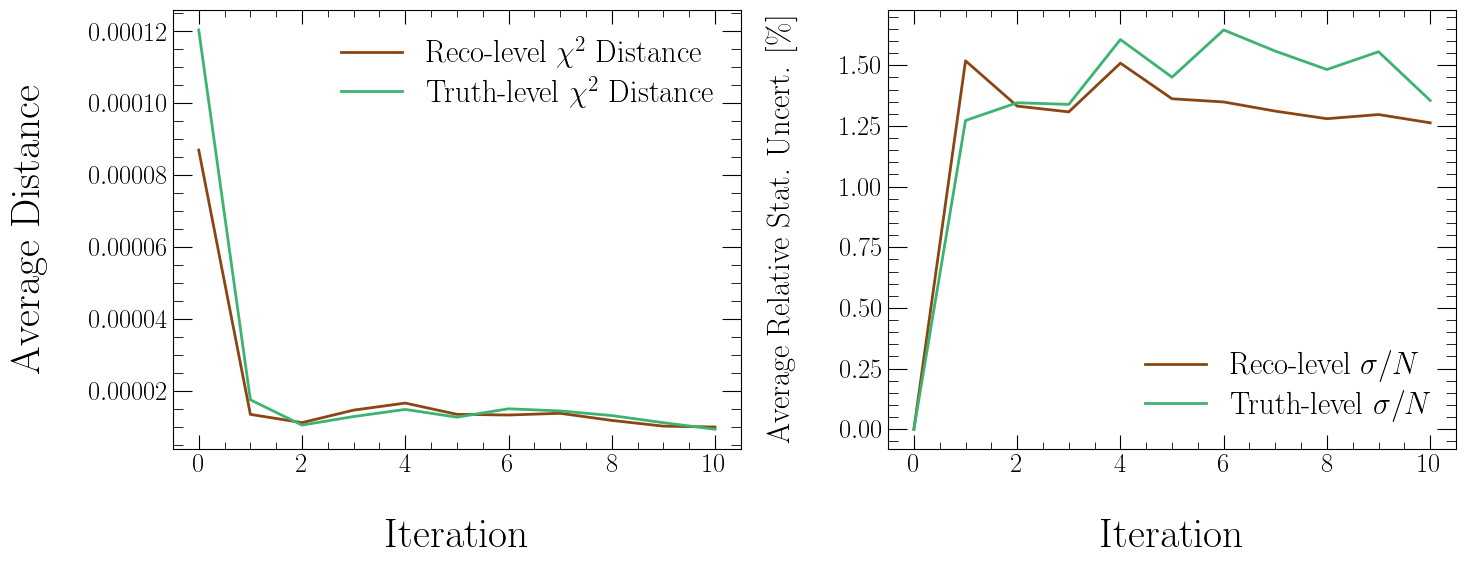
\includegraphics[width=0.95\textwidth]{figures/num_iterations_study/Ntracks_trackj1/iteration_study_30x10-distances-and-stat-uncert.png}\\
\caption{\textbf{Leading jet $n_{\text{charged tracks}}$:} On the left, average $\chi^2$ histogram distance per iteration, and on the right, average relative statistical uncertainty per iteration.}
\label{fig:num_iterations:ntracks_distances_stat_uncert}
\end{figure}
\begin{figure}[!htb]
\centering
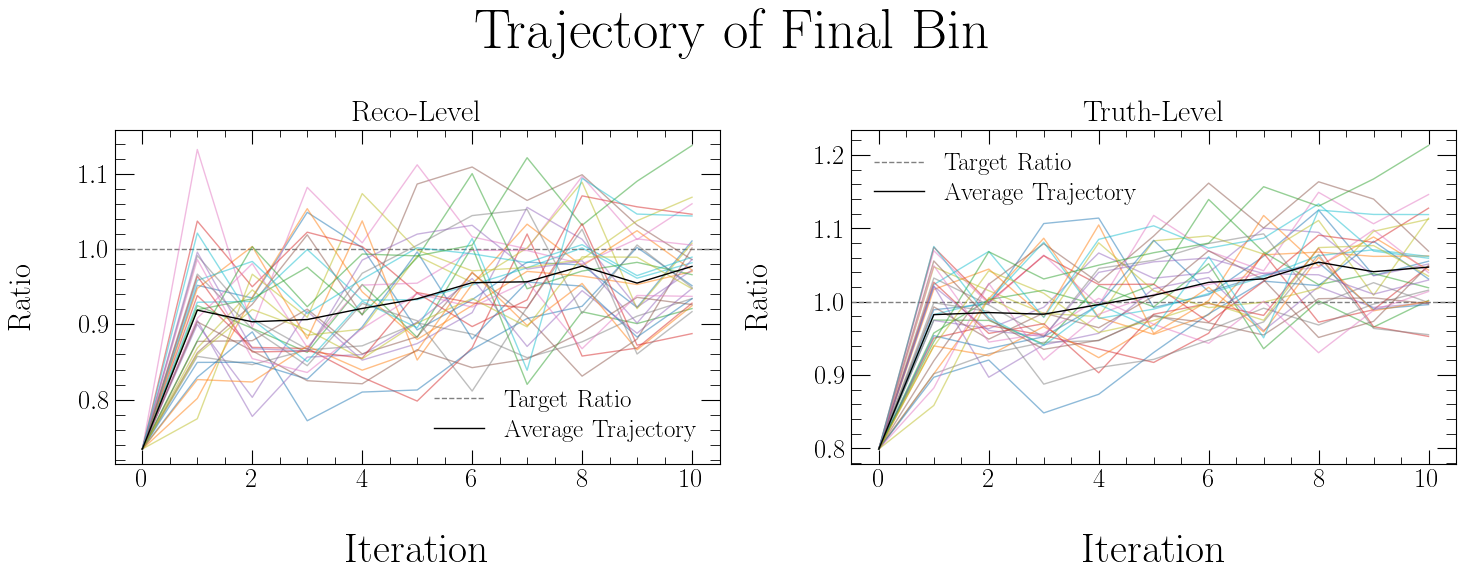
\includegraphics[width=0.95\textwidth]{figures/num_iterations_study/Ntracks_trackj1/iteration_study_30x10-final_bin.png}\\
\caption{\textbf{Leading jet $n_{\text{charged tracks}}$:} Trajectories of the final bin for each of the 30 bootstrapped independent trials as well as the average trajectory. The ratio is the unfolded histogram with respect to the target histogram.}
\label{fig:num_iterations:ntracks_final_bin}
\end{figure}


\subsection{Leading jet $p_T$}
\subsubsection{Ratios of unfolded histograms for one trial}
\begin{figure}[]
\centering
\subfloat[Iteration 0 (before unfolding/bootstrapping)]{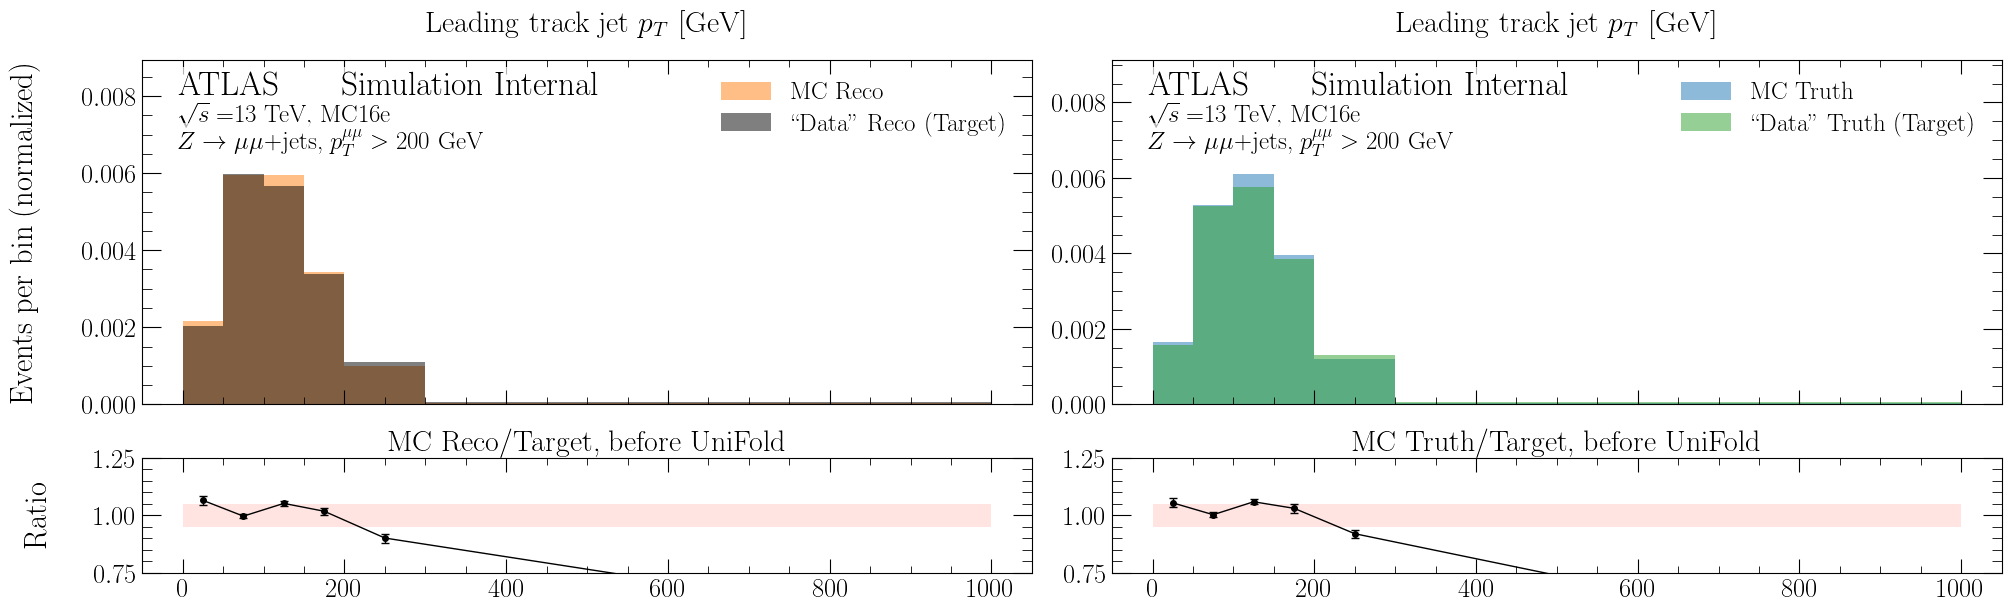
\includegraphics[width=0.95\textwidth]{figures/num_iterations_study/pT_trackj1/iteration_study_30x10-Iteration00.png}}\\
\subfloat[Iteration 1]{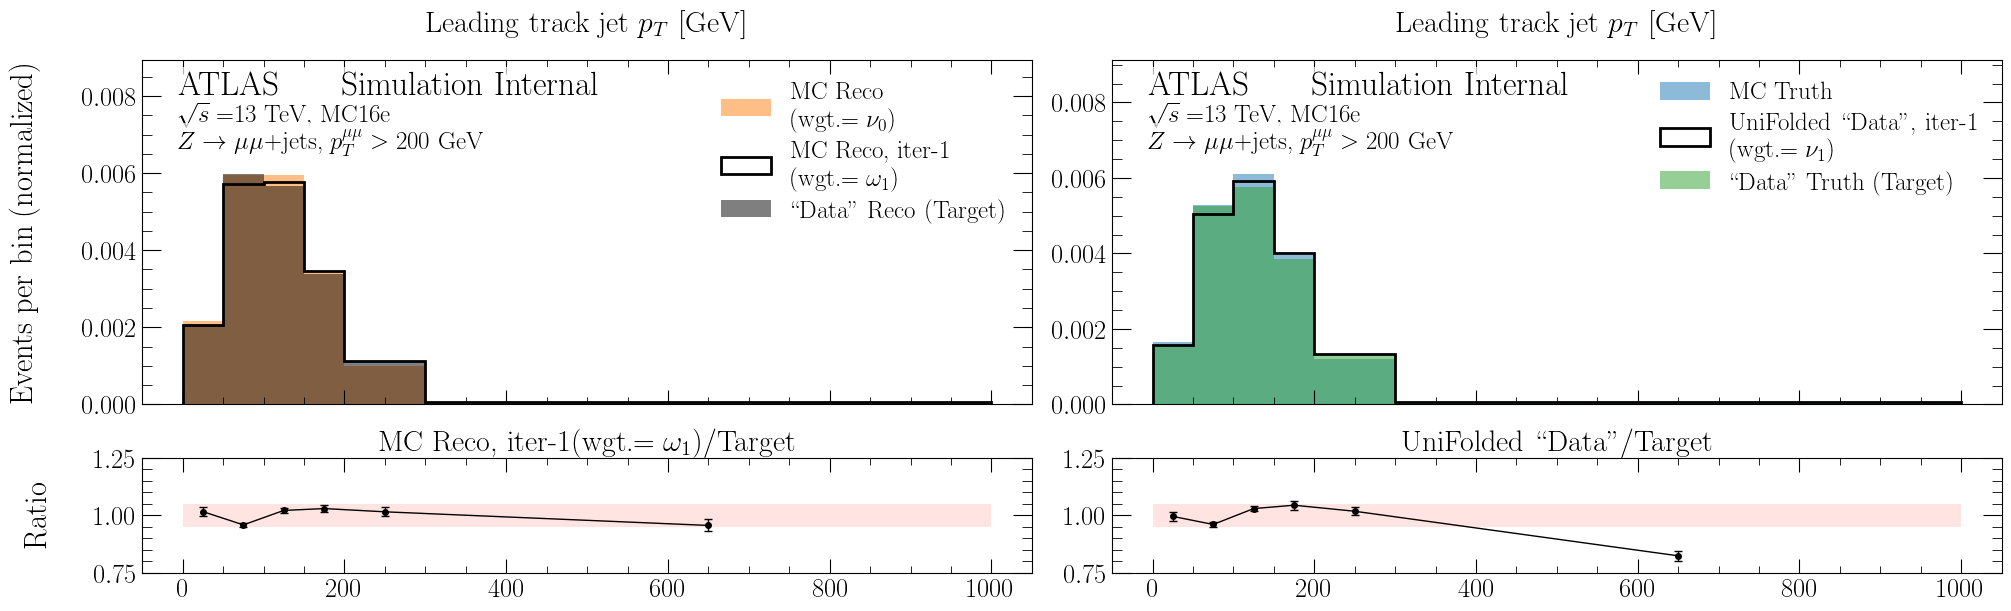
\includegraphics[width=0.95\textwidth]{figures/num_iterations_study/pT_trackj1/iteration_study_30x10-Iteration01.png}}\\
\subfloat[Iteration 2]{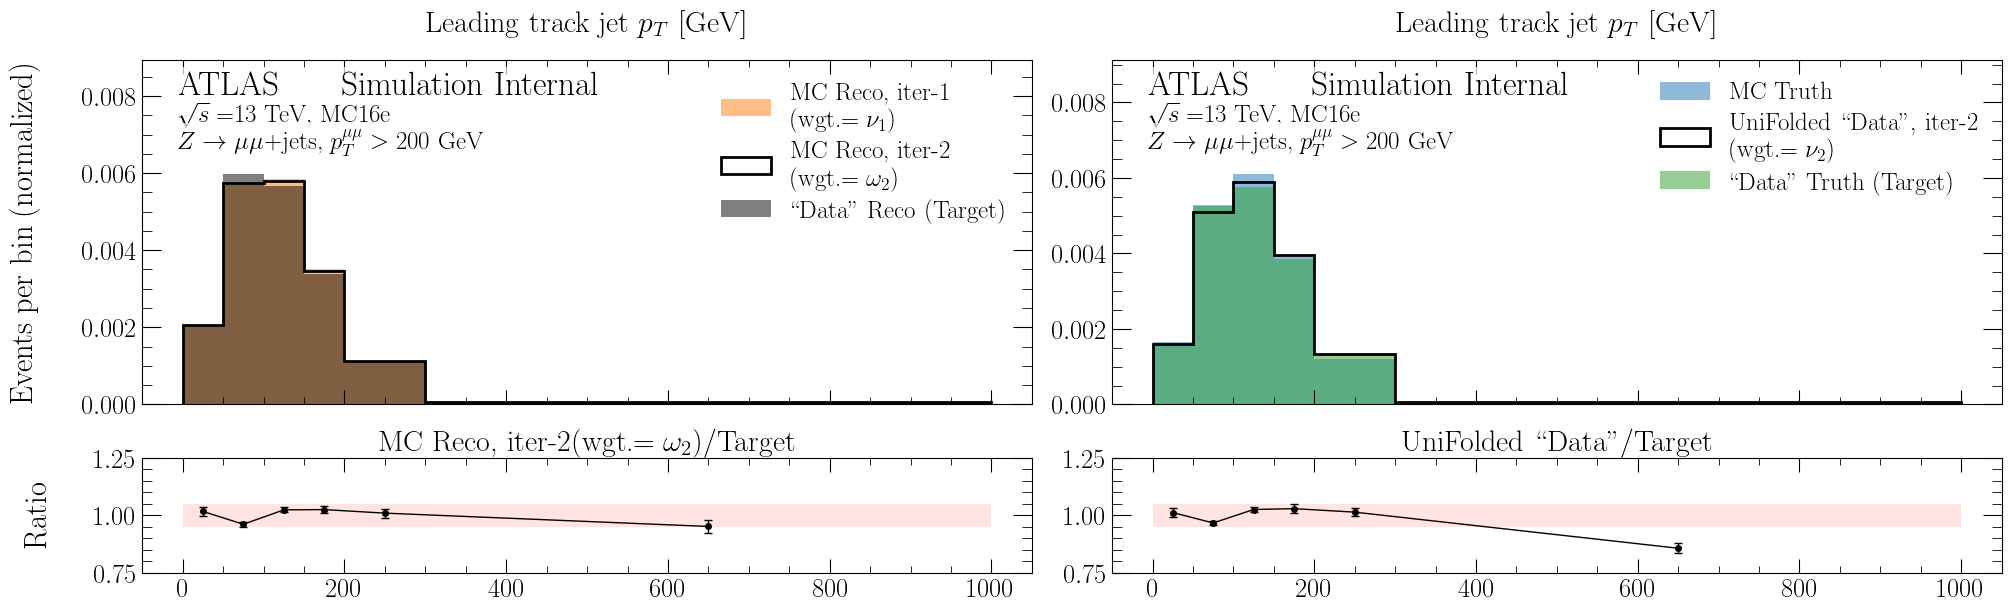
\includegraphics[width=0.95\textwidth]{figures/num_iterations_study/pT_trackj1/iteration_study_30x10-Iteration02.png}}\\
\subfloat[Iteration 3]{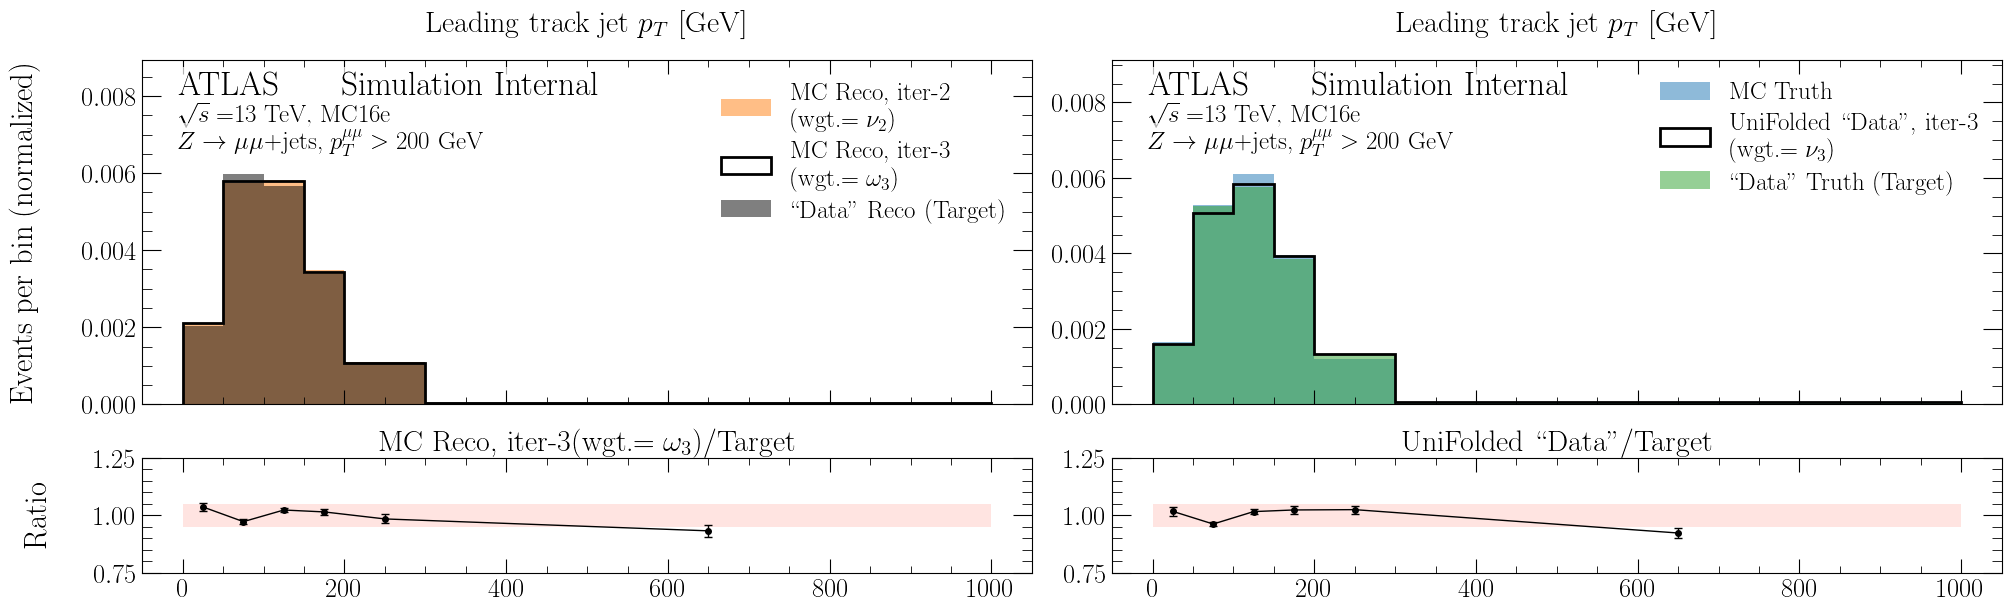
\includegraphics[width=0.95\textwidth]{figures/num_iterations_study/pT_trackj1/iteration_study_30x10-Iteration03.png}}
\phantomcaption
\end{figure}
\begin{figure}[]
\centering
\ContinuedFloat
\subfloat[Iteration 4]{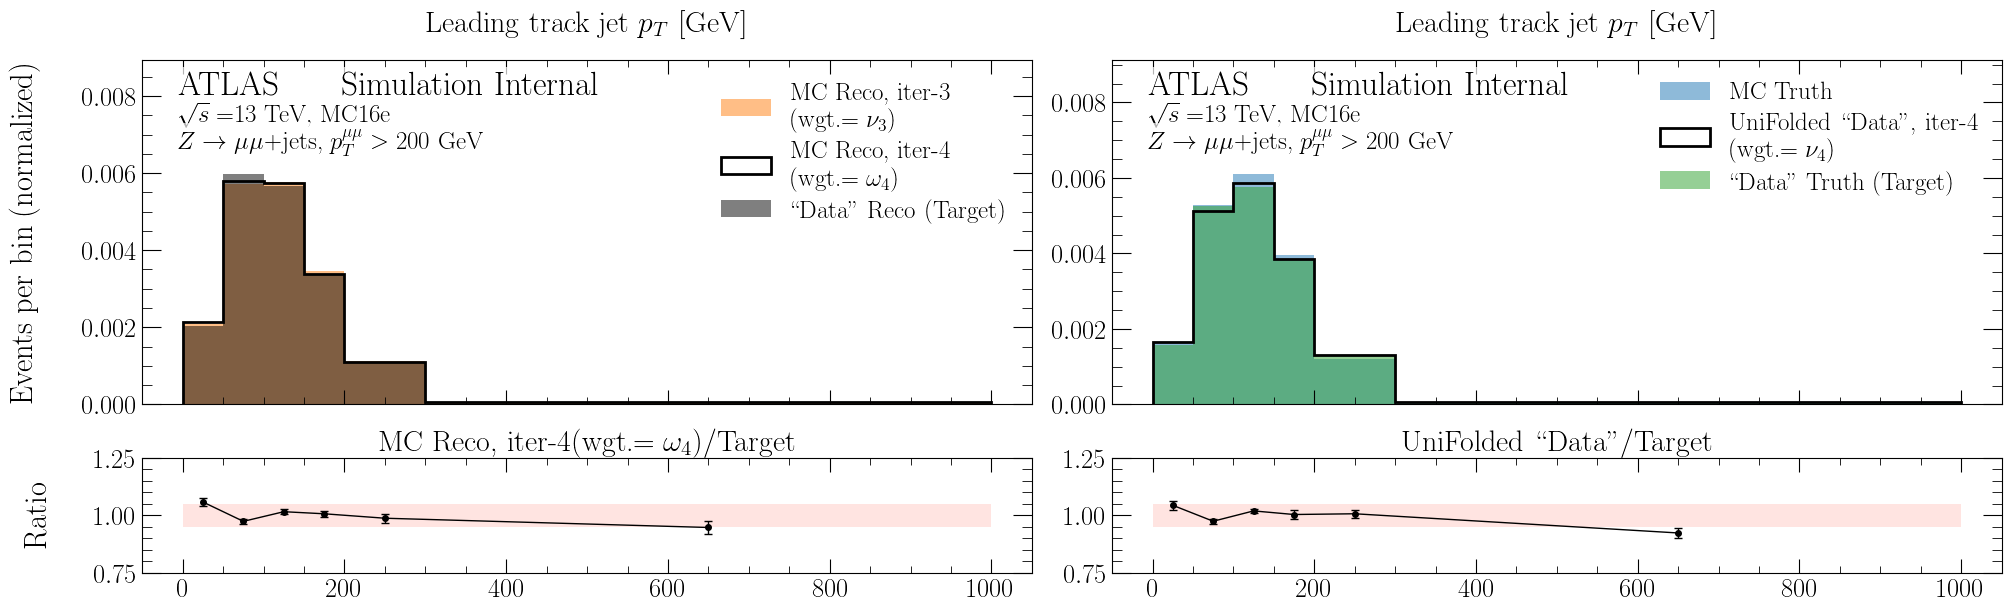
\includegraphics[width=0.95\textwidth]{figures/num_iterations_study/pT_trackj1/iteration_study_30x10-Iteration04.png}}\\
\subfloat[Iteration 5]{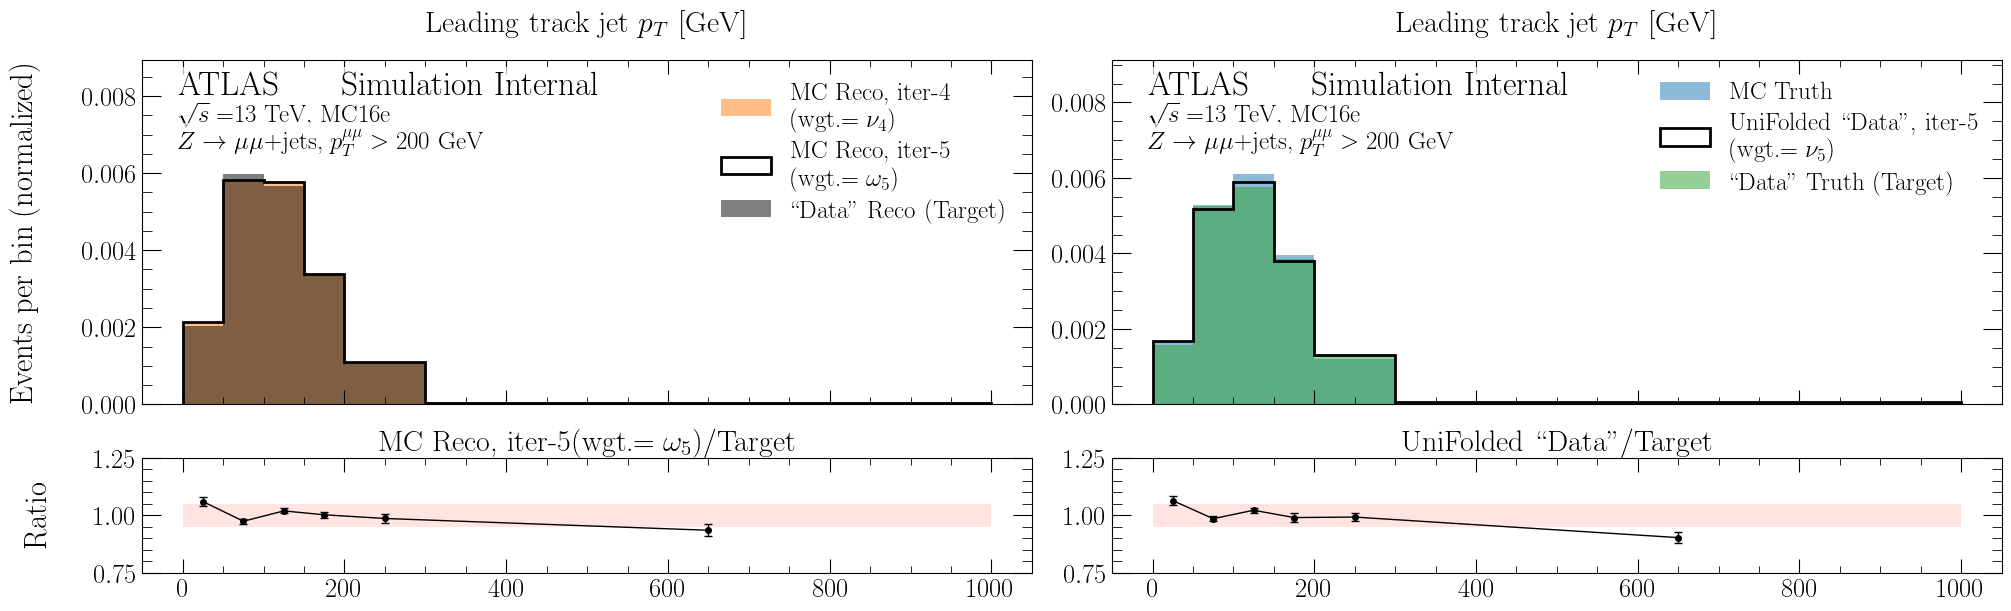
\includegraphics[width=0.95\textwidth]{figures/num_iterations_study/pT_trackj1/iteration_study_30x10-Iteration05.png}}\\
\subfloat[Iteration 6]{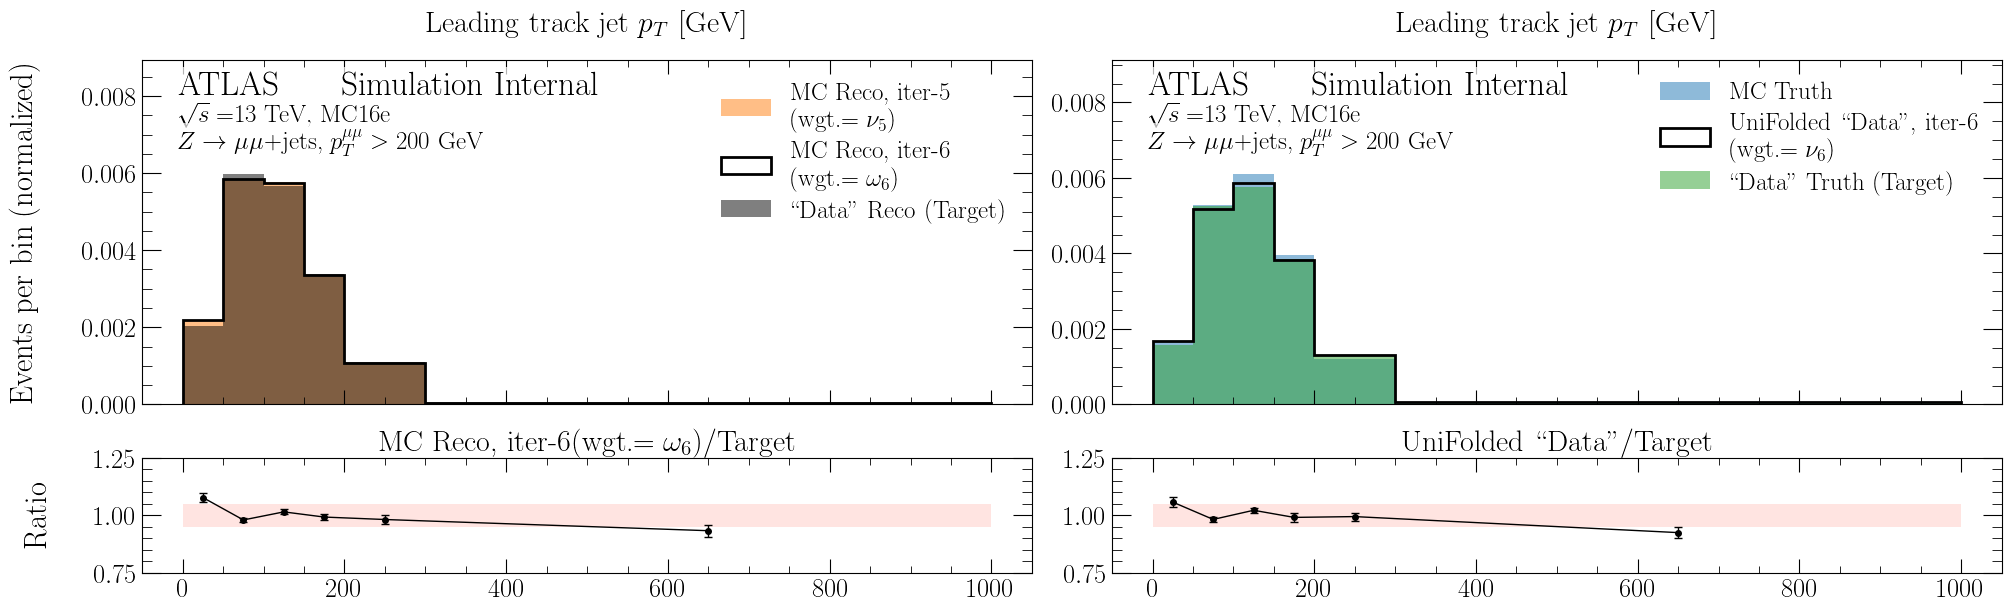
\includegraphics[width=0.95\textwidth]{figures/num_iterations_study/pT_trackj1/iteration_study_30x10-Iteration06.png}}\\
\subfloat[Iteration 7]{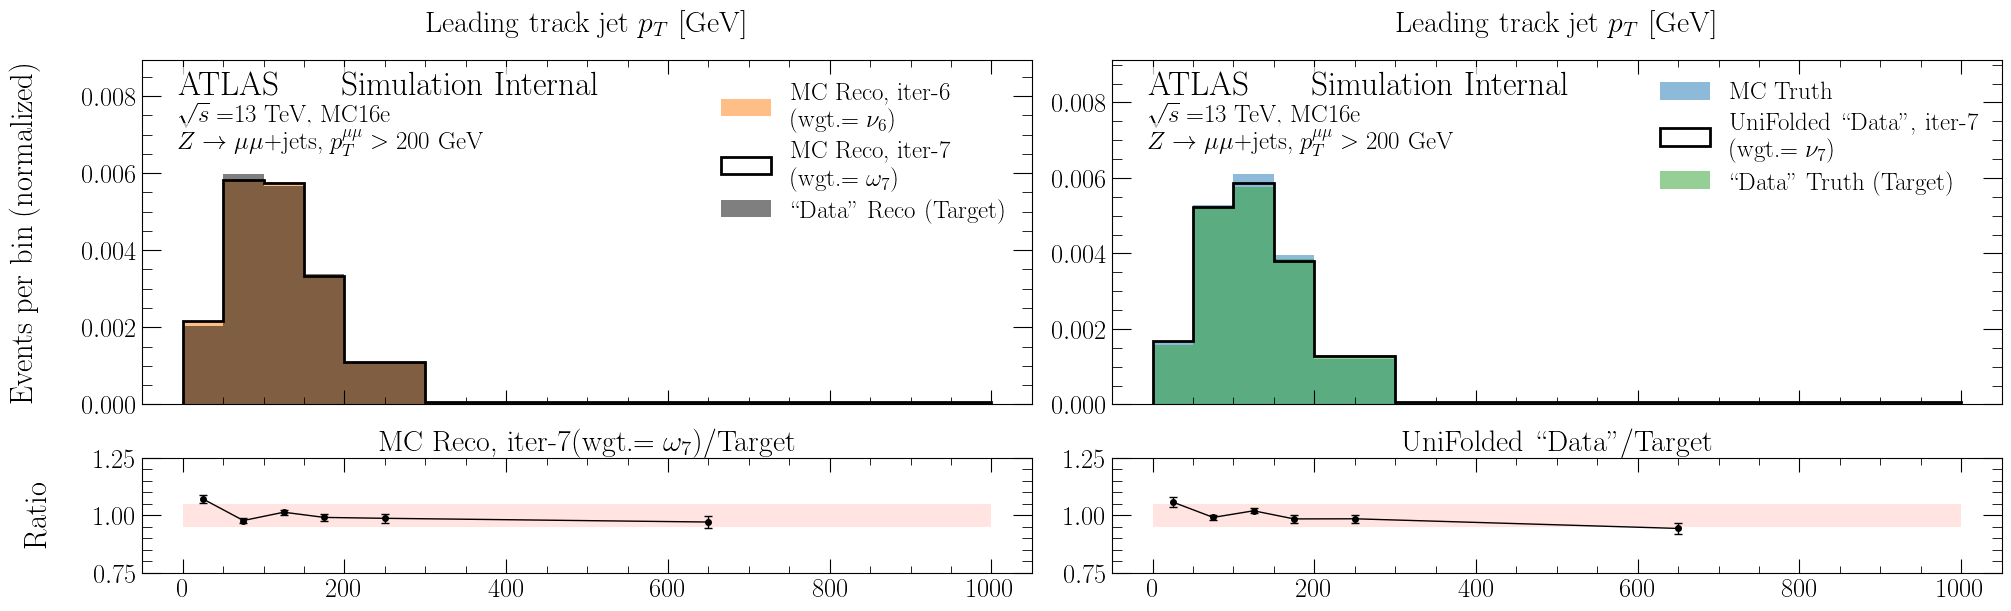
\includegraphics[width=0.95\textwidth]{figures/num_iterations_study/pT_trackj1/iteration_study_30x10-Iteration07.png}}
\phantomcaption
\end{figure}
\begin{figure}[]
\centering
\ContinuedFloat
\subfloat[Iteration 8]{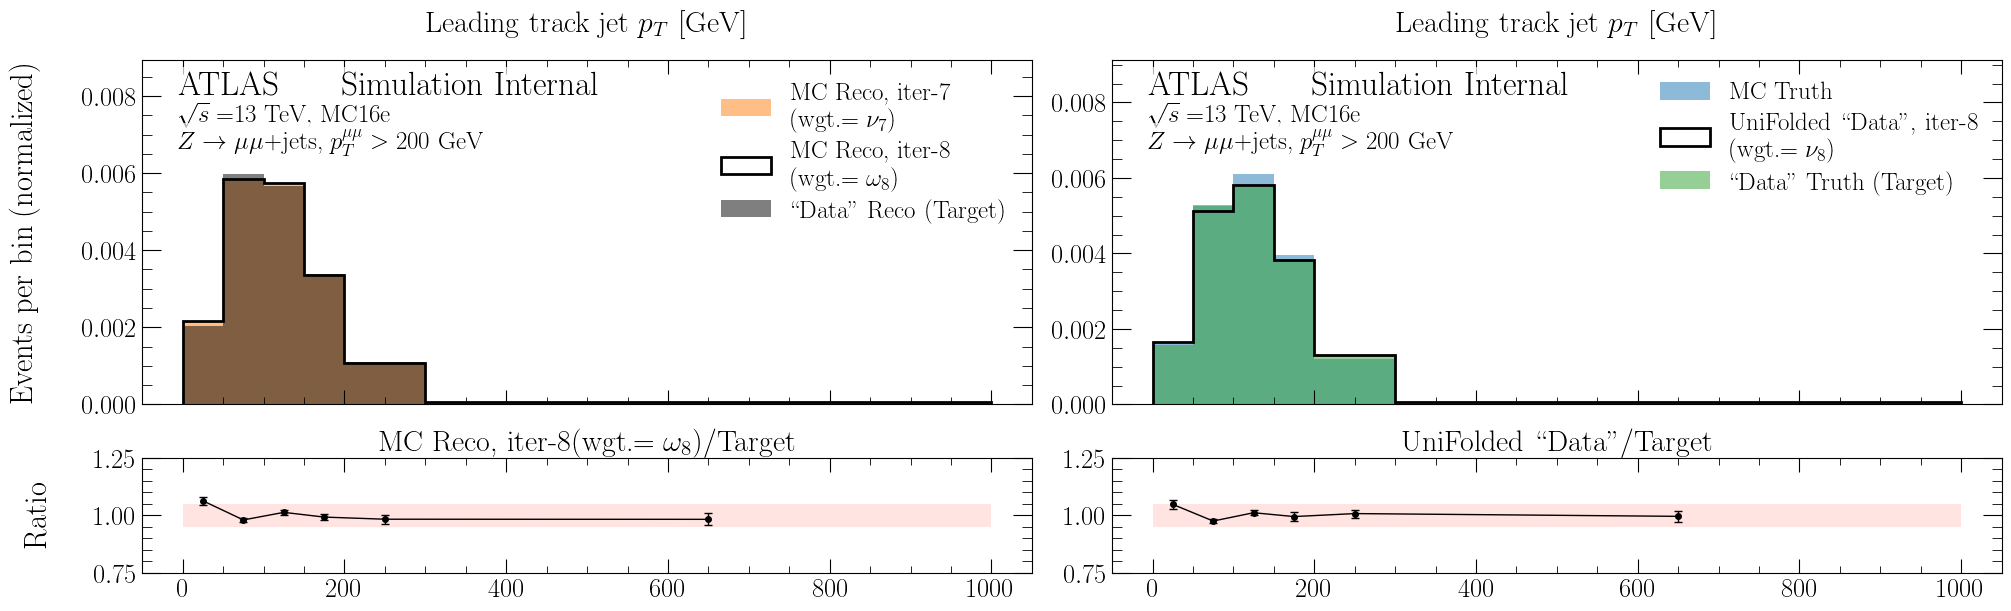
\includegraphics[width=0.95\textwidth]{figures/num_iterations_study/pT_trackj1/iteration_study_30x10-Iteration08.png}}\\
\subfloat[Iteration 9]{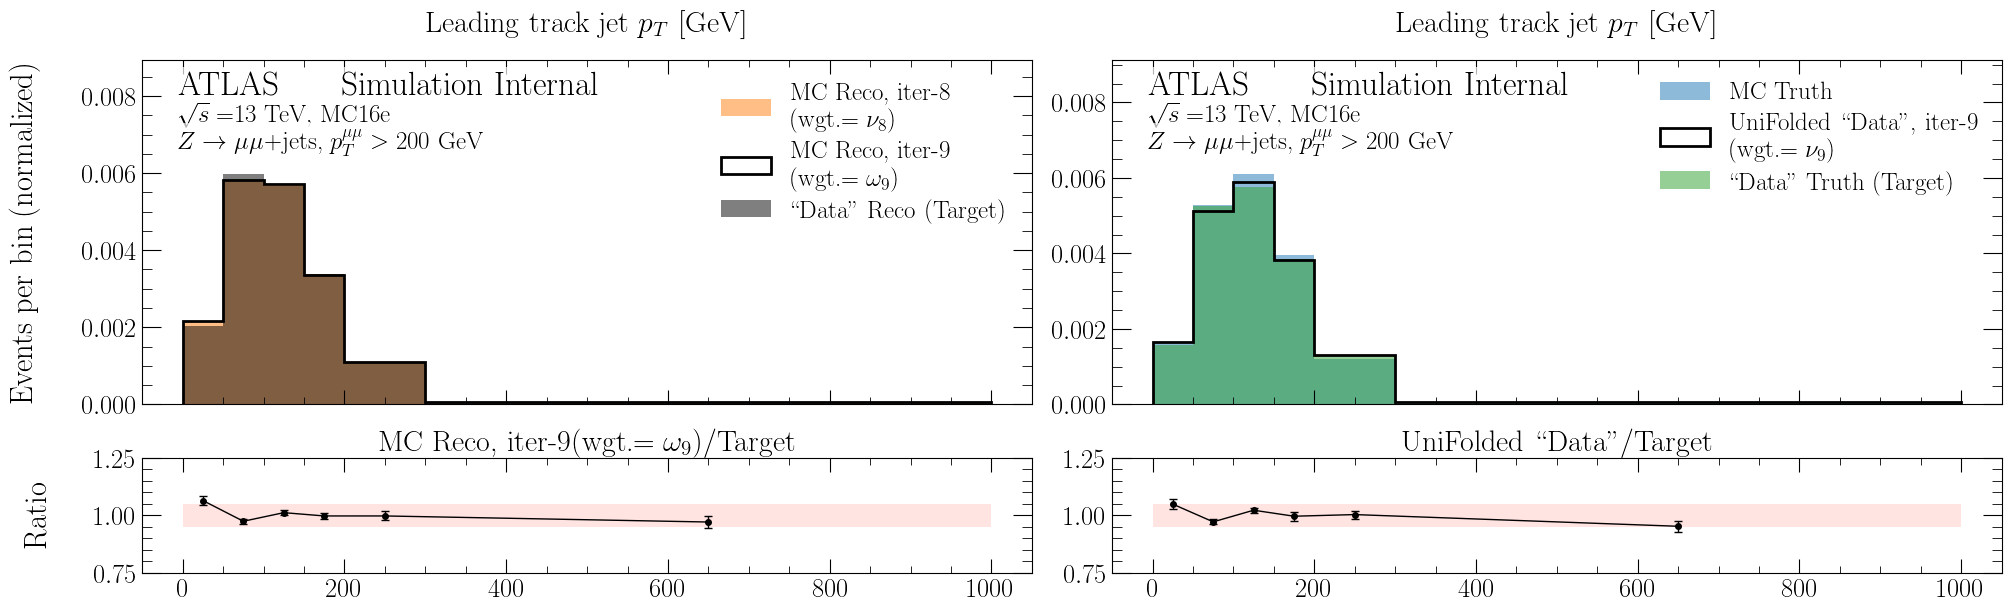
\includegraphics[width=0.95\textwidth]{figures/num_iterations_study/pT_trackj1/iteration_study_30x10-Iteration09.png}}\\
\subfloat[Iteration 10]{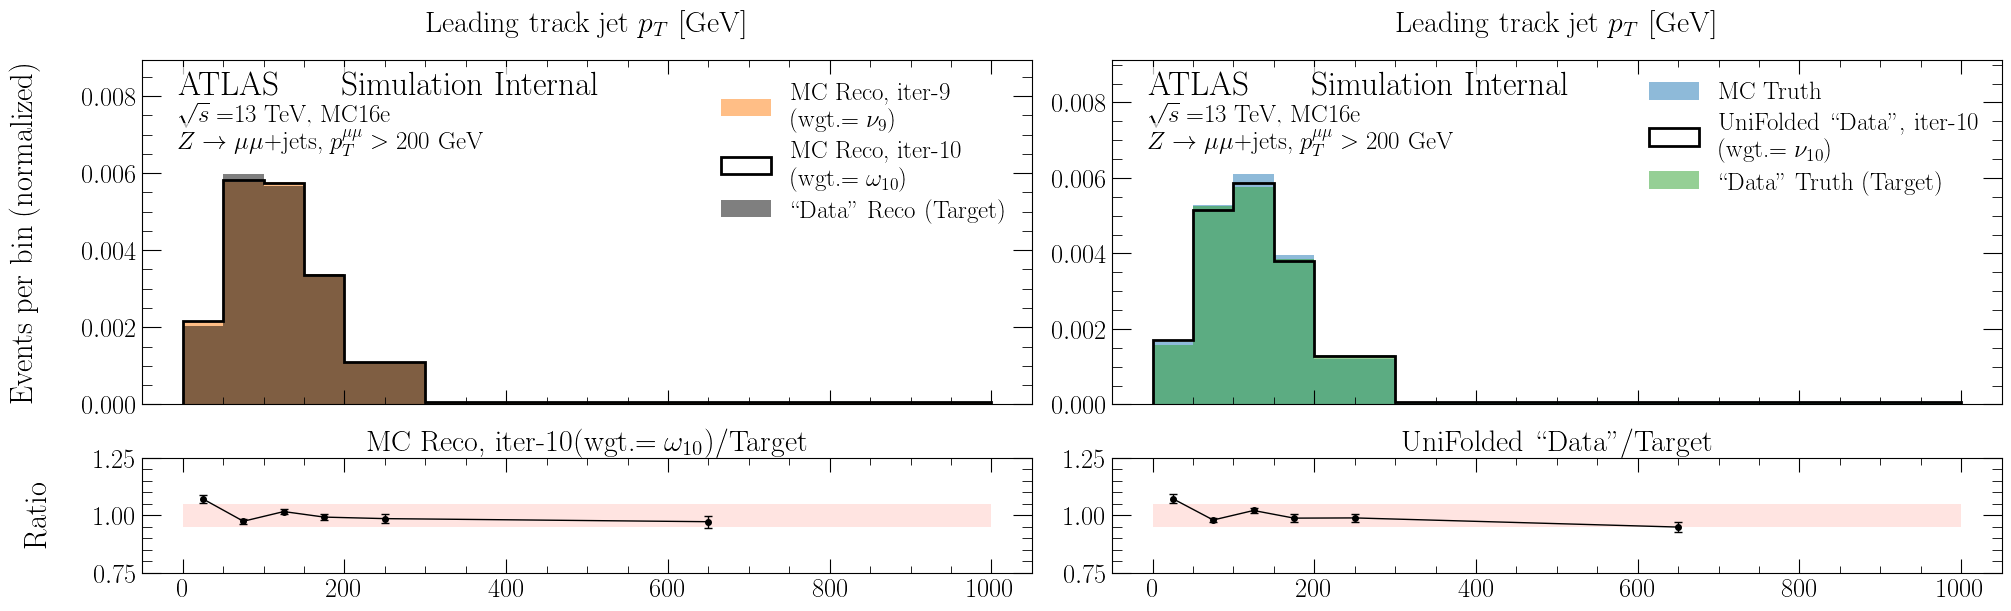
\includegraphics[width=0.95\textwidth]{figures/num_iterations_study/pT_trackj1/iteration_study_30x10-Iteration10.png}}
\caption{\textbf{Leading jet $\p_T$:} The unfolded histograms for UniFold in a single trial with Poisson bootstrapping applied. The ratio plots reveal that the bulk of the distribution quickly achieves good performance after about two iterations, but the tails of the distribution can sometimes benefit from additional iterations.}
\label{fig:num_iterations:pT_ratios}
\end{figure}


\subsubsection{Performance as a function of iteration}
\begin{figure}[!htb]
\centering
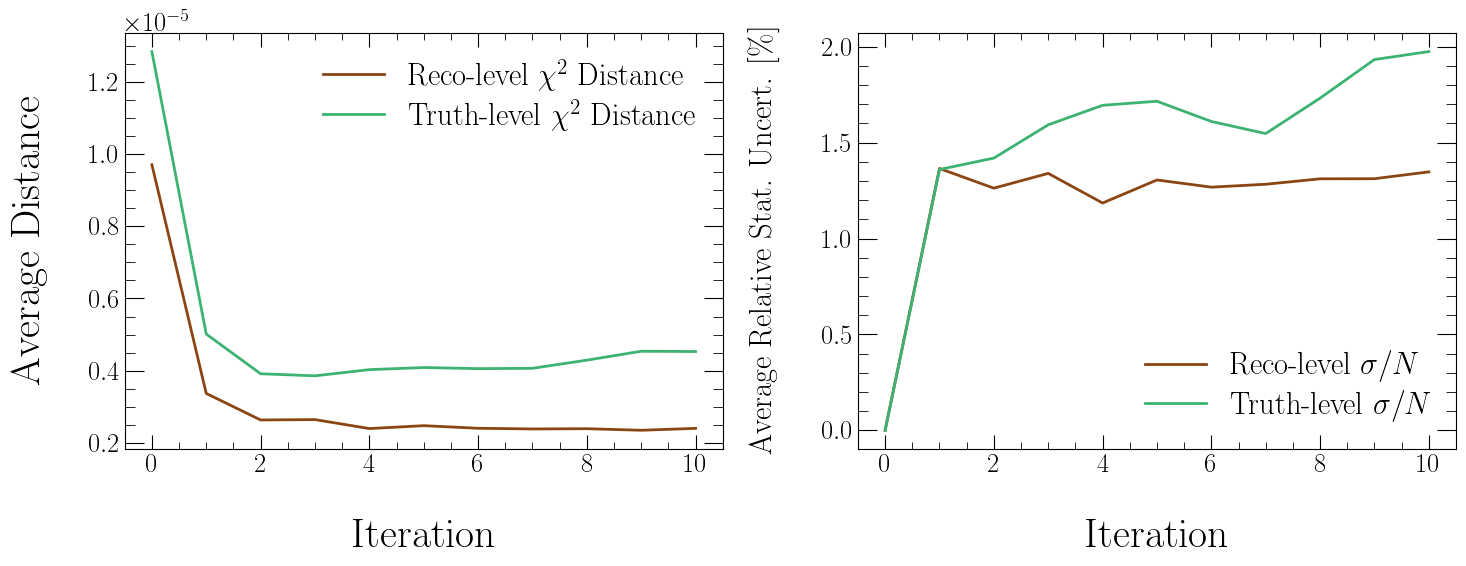
\includegraphics[width=0.95\textwidth]{figures/num_iterations_study/pT_trackj1/iteration_study_30x10-distances-and-stat-uncert.png}\\
\caption{\textbf{Leading jet $p_T$:} On the left, average $\chi^2$ histogram distance per iteration, and on the right, average relative statistical uncertainty per iteration.}
\label{fig:num_iterations:pT_distances_stat_uncert}
\end{figure}
\begin{figure}[!htb]
\centering
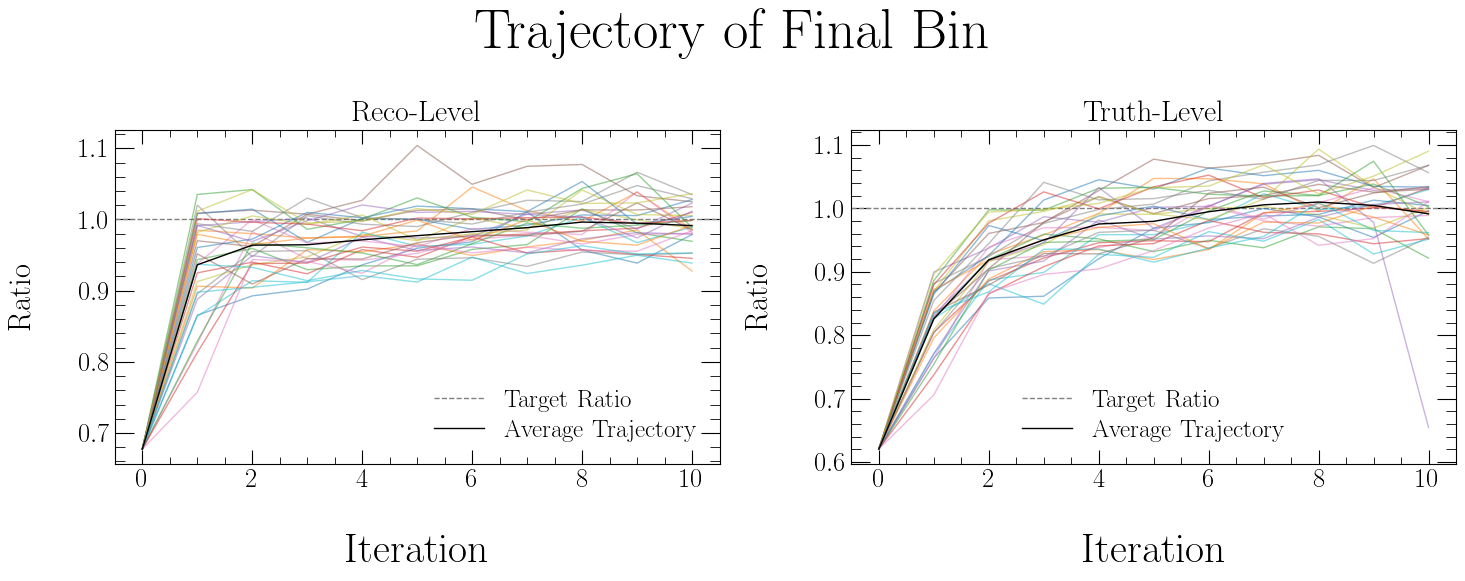
\includegraphics[width=0.95\textwidth]{figures/num_iterations_study/pT_trackj1/iteration_study_30x10-final_bin.png}\\
\caption{\textbf{Leading jet $\p_T$:} Trajectories of the final bin for each of the 30 bootstrapped independent trials as well as the average trajectory. The ratio is the unfolded histogram with respect to the target histogram.}
\label{fig:num_iterations:pT_final_bin}
\end{figure}

\subsection{Leading jet $\tau_1$}
\subsubsection{Ratios of unfolded histograms for one trial}
\begin{figure}[]
\centering
\subfloat[Iteration 0 (before unfolding/bootstrapping)]{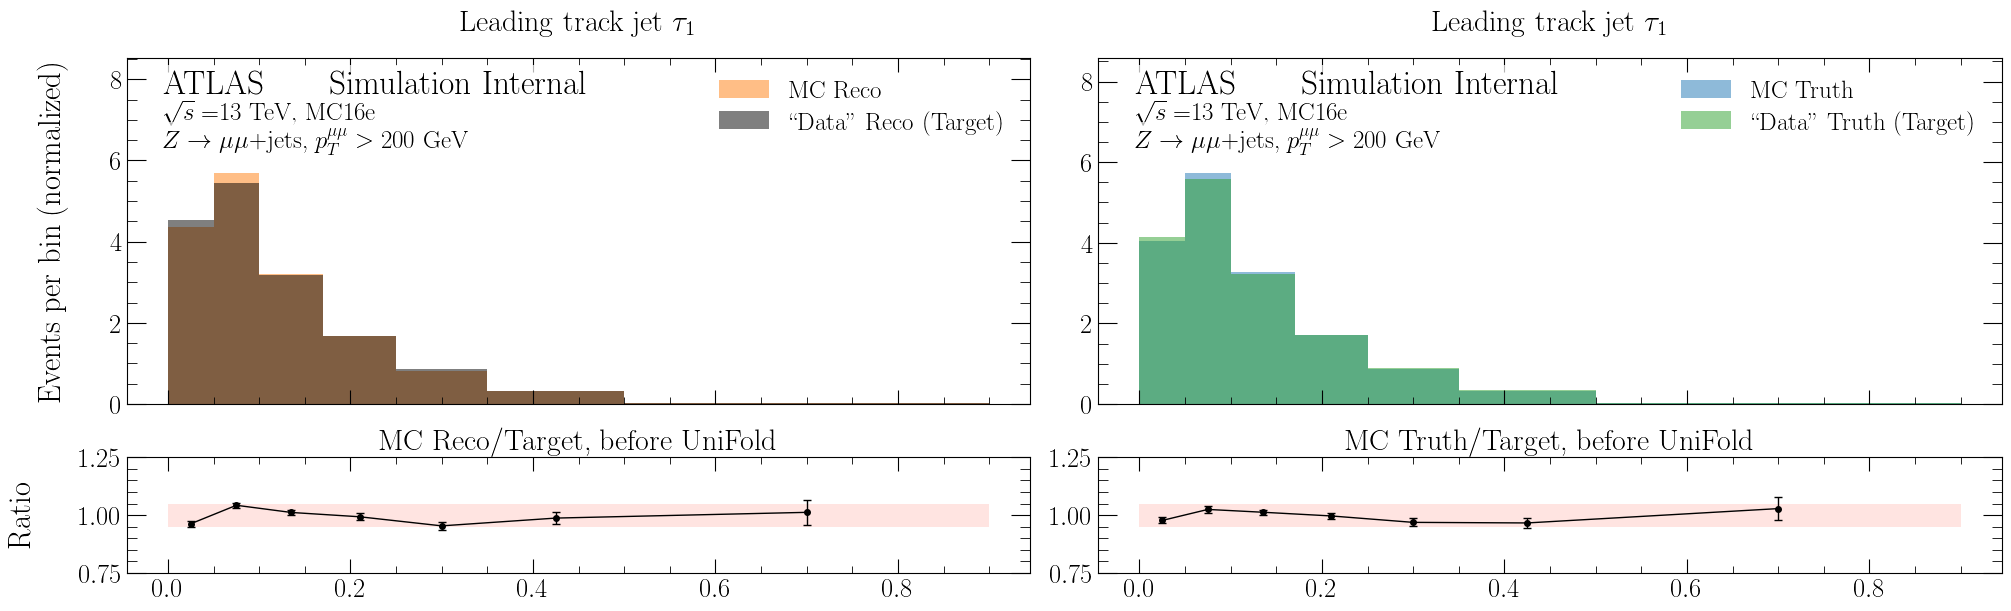
\includegraphics[width=0.95\textwidth]{figures/num_iterations_study/tau1_trackj1/iteration_study_30x10-Iteration00.png}}\\
\subfloat[Iteration 1]{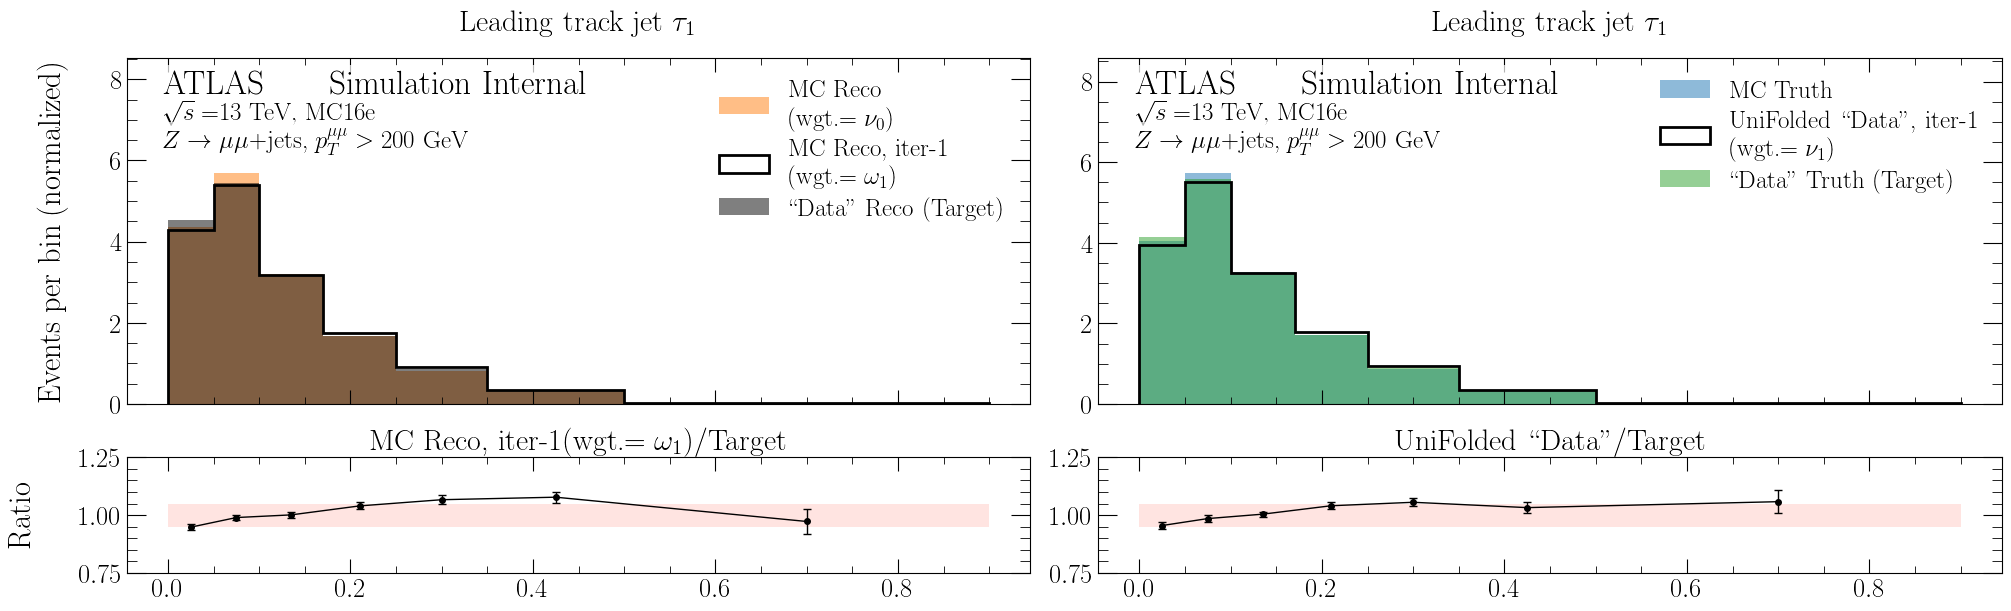
\includegraphics[width=0.95\textwidth]{figures/num_iterations_study/tau1_trackj1/iteration_study_30x10-Iteration01.png}}\\
\subfloat[Iteration 2]{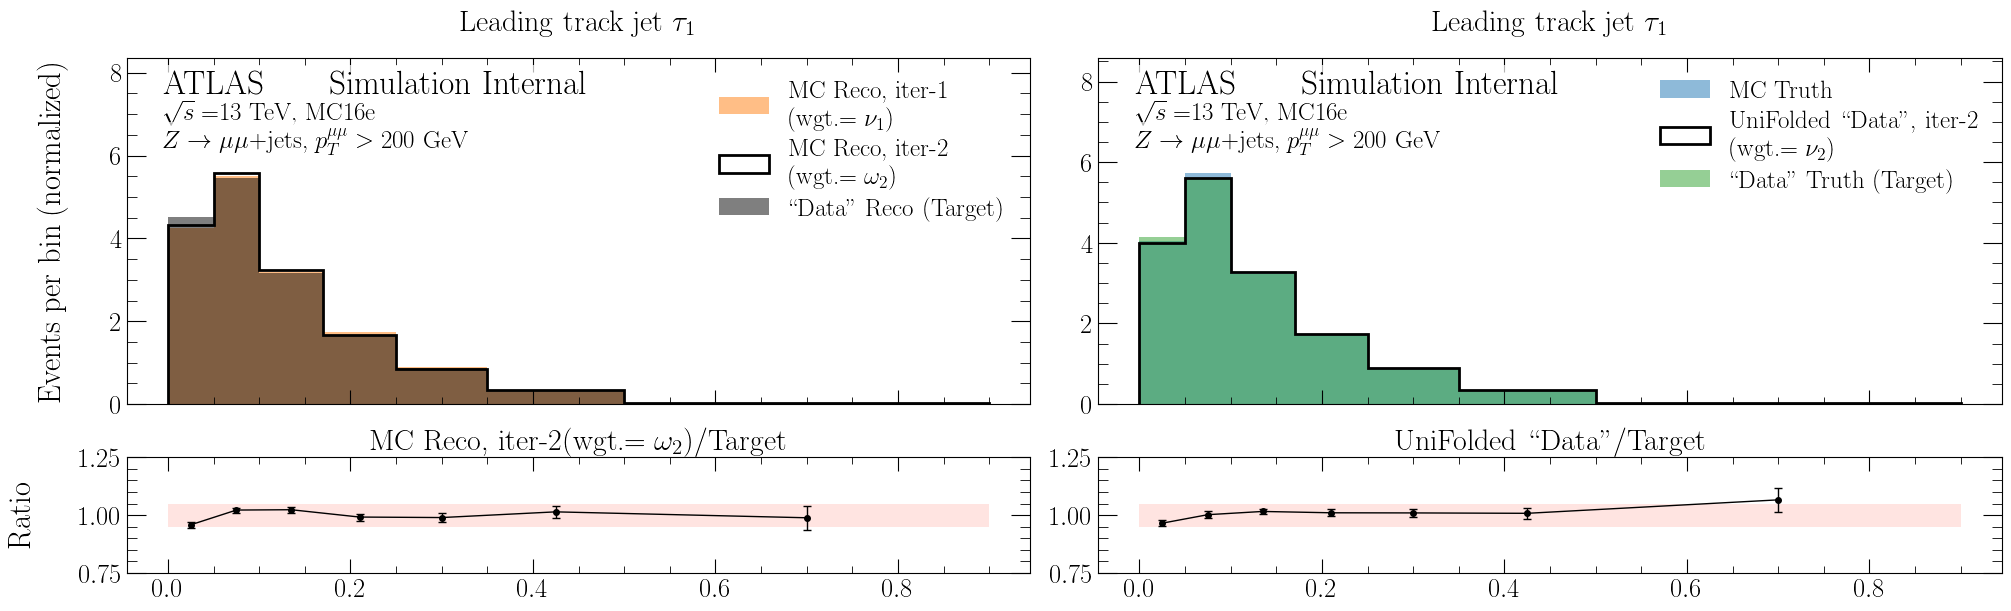
\includegraphics[width=0.95\textwidth]{figures/num_iterations_study/tau1_trackj1/iteration_study_30x10-Iteration02.png}}\\
\subfloat[Iteration 3]{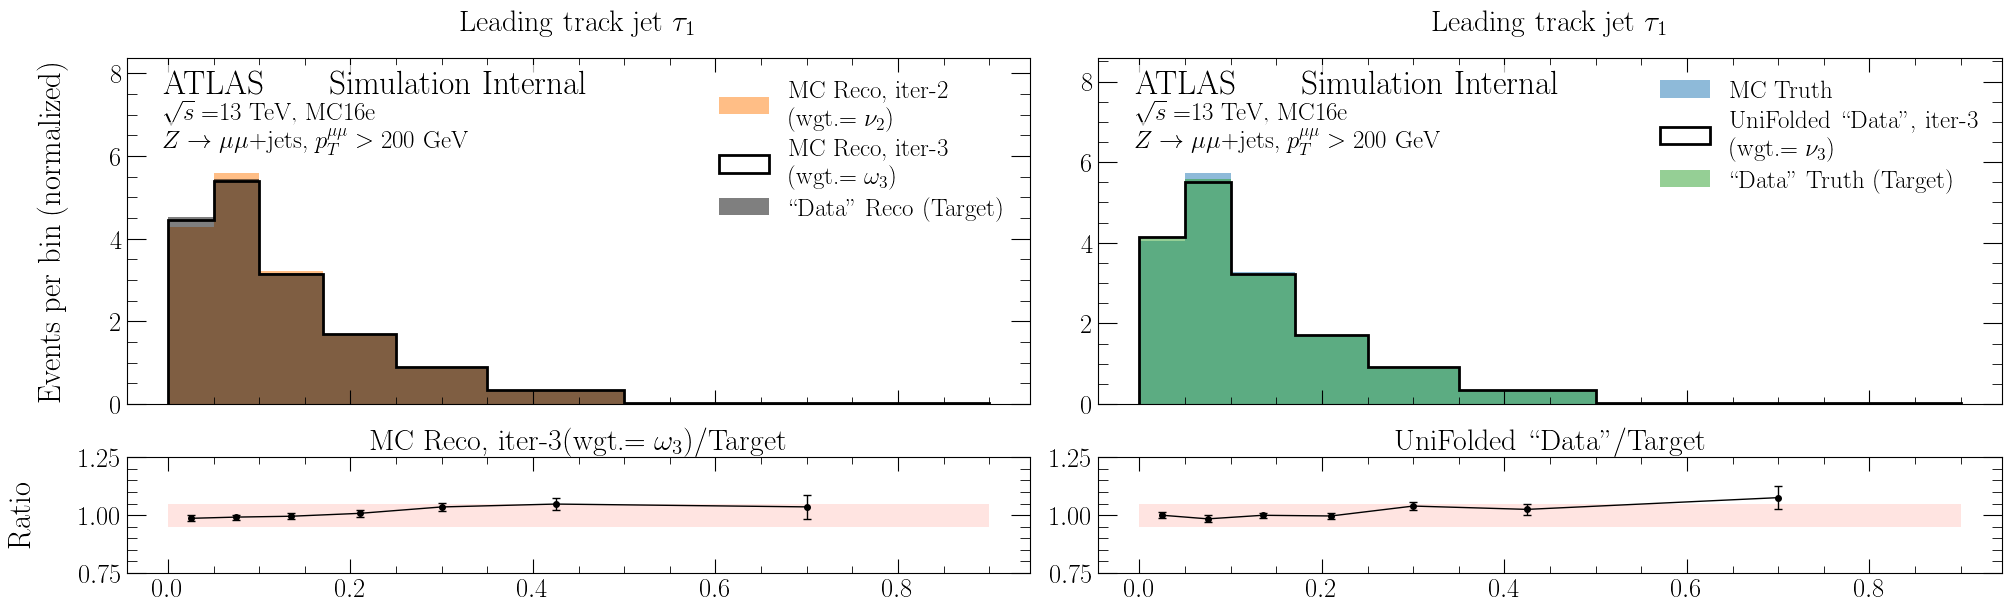
\includegraphics[width=0.95\textwidth]{figures/num_iterations_study/tau1_trackj1/iteration_study_30x10-Iteration03.png}}
\phantomcaption
\end{figure}
\begin{figure}[]
\centering
\ContinuedFloat
\subfloat[Iteration 4]{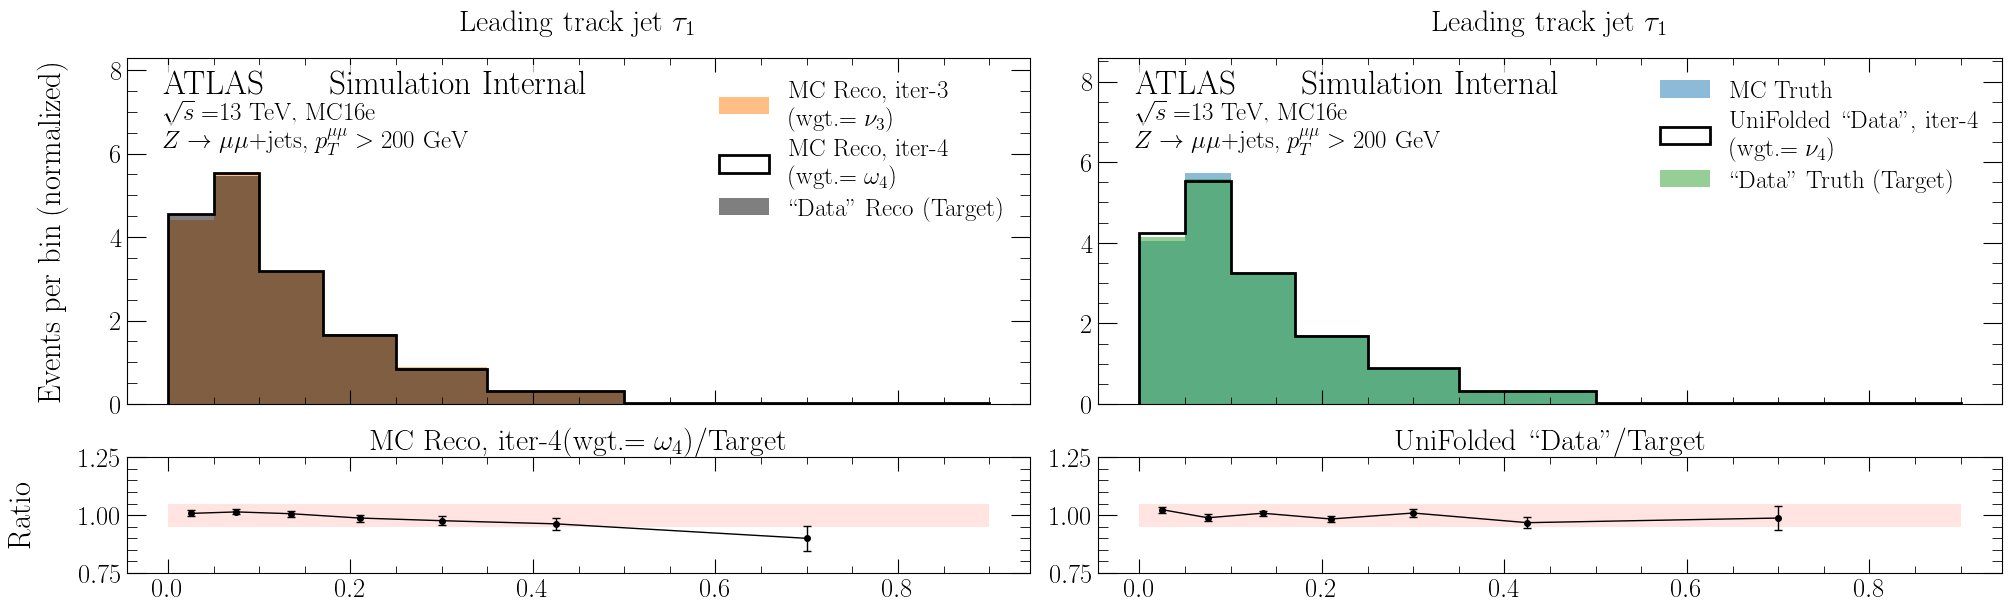
\includegraphics[width=0.95\textwidth]{figures/num_iterations_study/tau1_trackj1/iteration_study_30x10-Iteration04.png}}\\
\subfloat[Iteration 5]{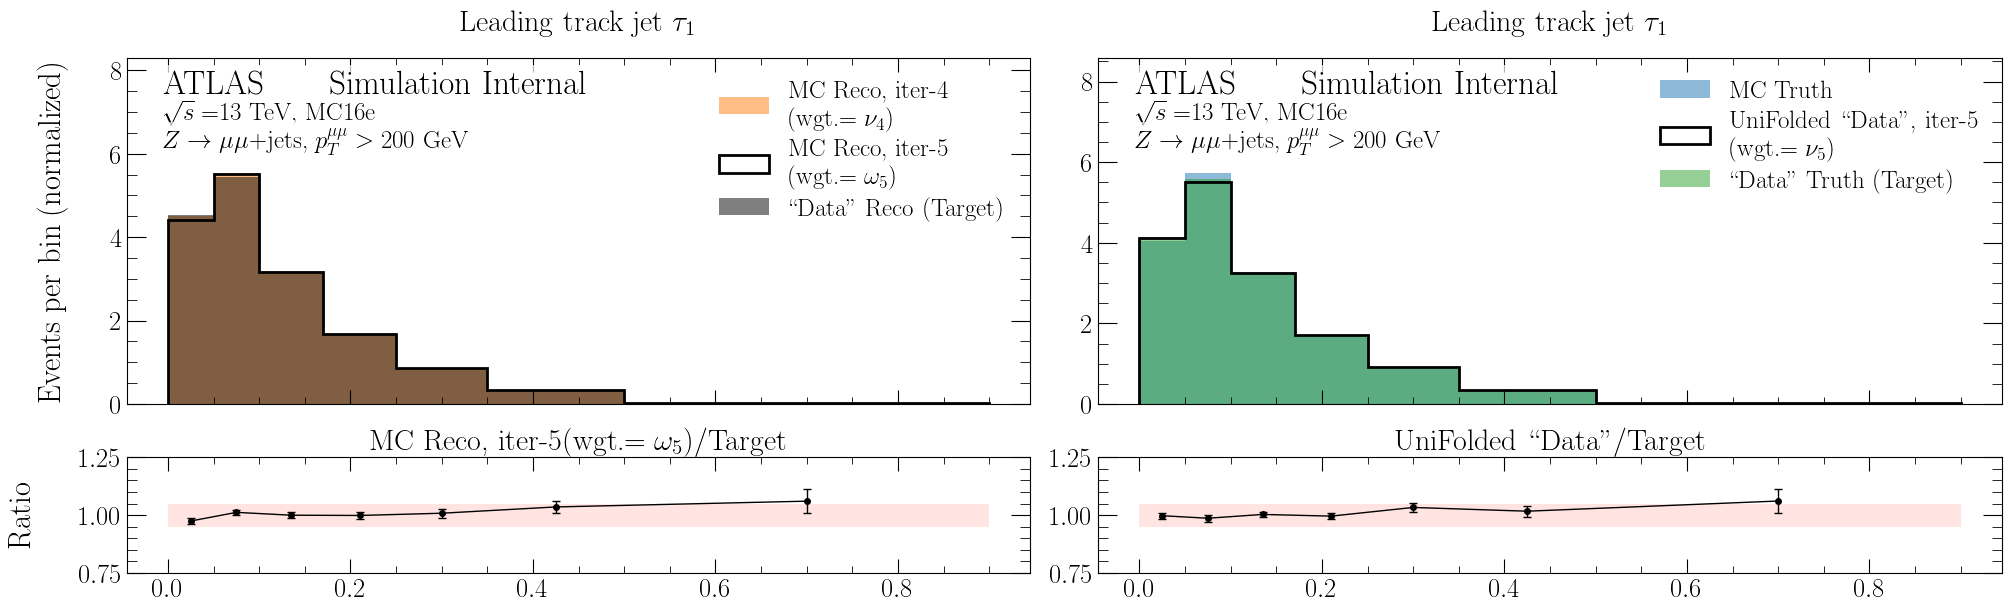
\includegraphics[width=0.95\textwidth]{figures/num_iterations_study/tau1_trackj1/iteration_study_30x10-Iteration05.png}}\\
\subfloat[Iteration 6]{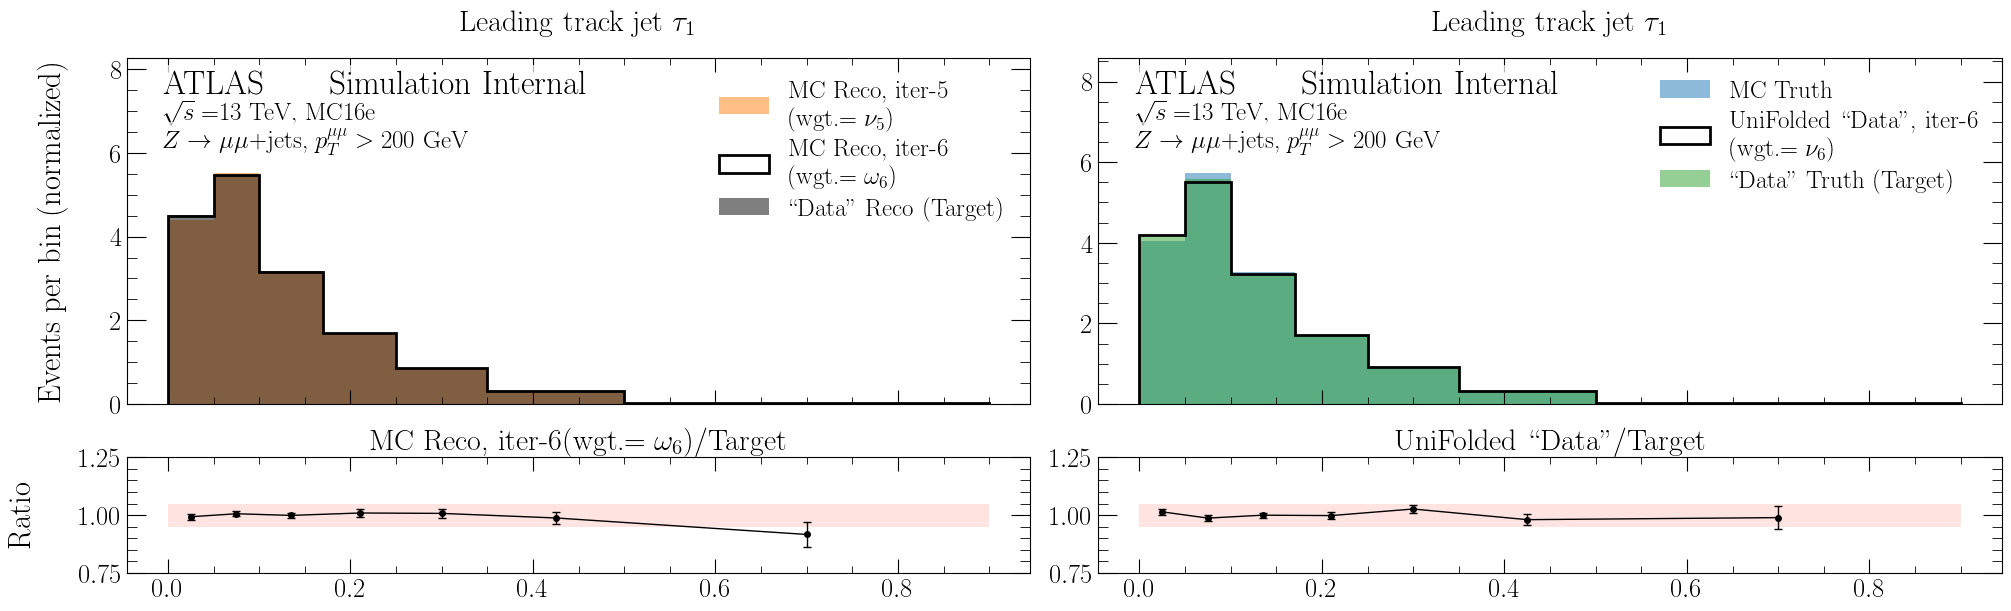
\includegraphics[width=0.95\textwidth]{figures/num_iterations_study/tau1_trackj1/iteration_study_30x10-Iteration06.png}}\\
\subfloat[Iteration 7]{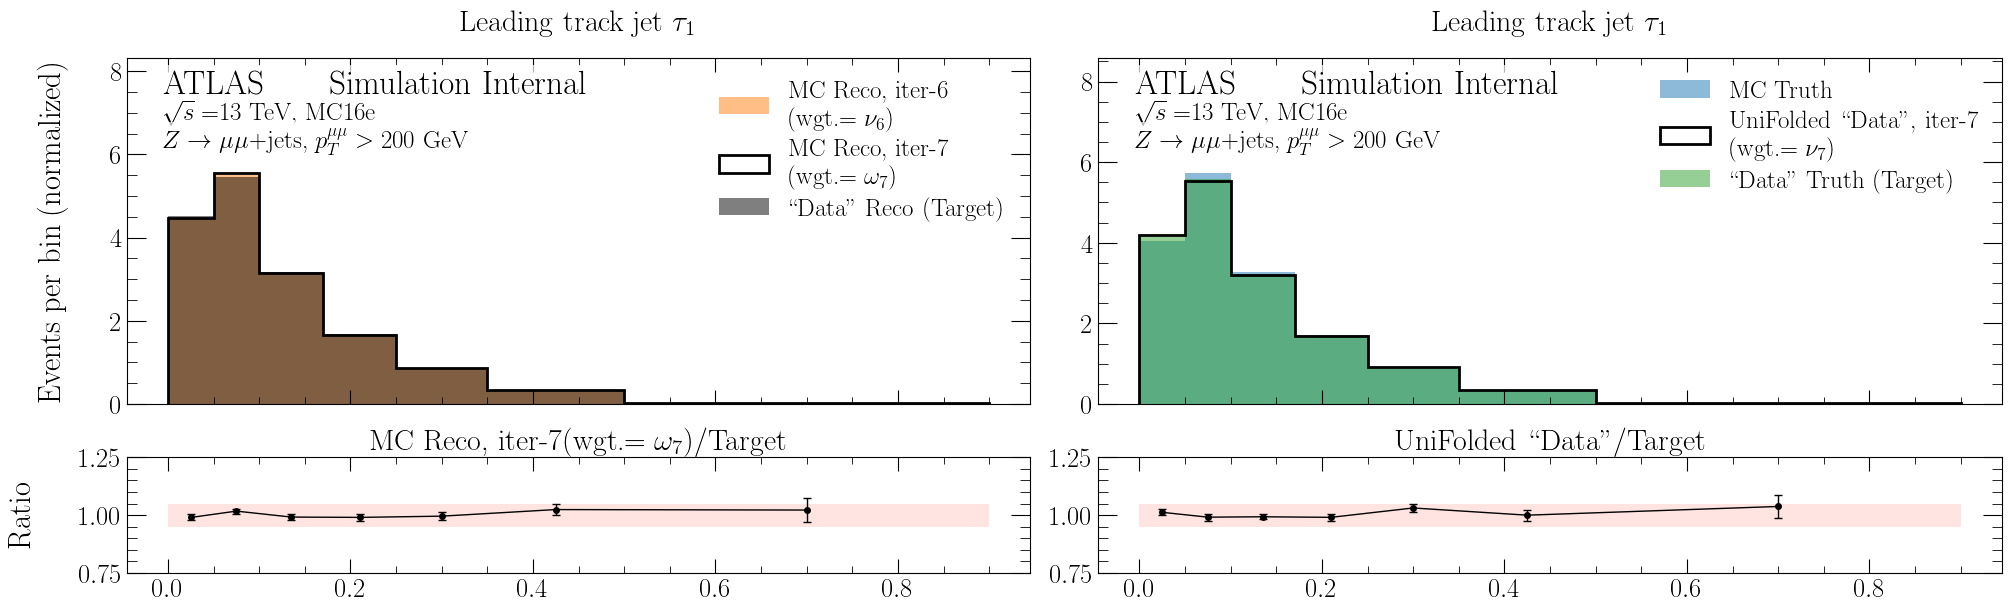
\includegraphics[width=0.95\textwidth]{figures/num_iterations_study/tau1_trackj1/iteration_study_30x10-Iteration07.png}}
\phantomcaption
\end{figure}
\begin{figure}[]
\centering
\ContinuedFloat
\subfloat[Iteration 8]{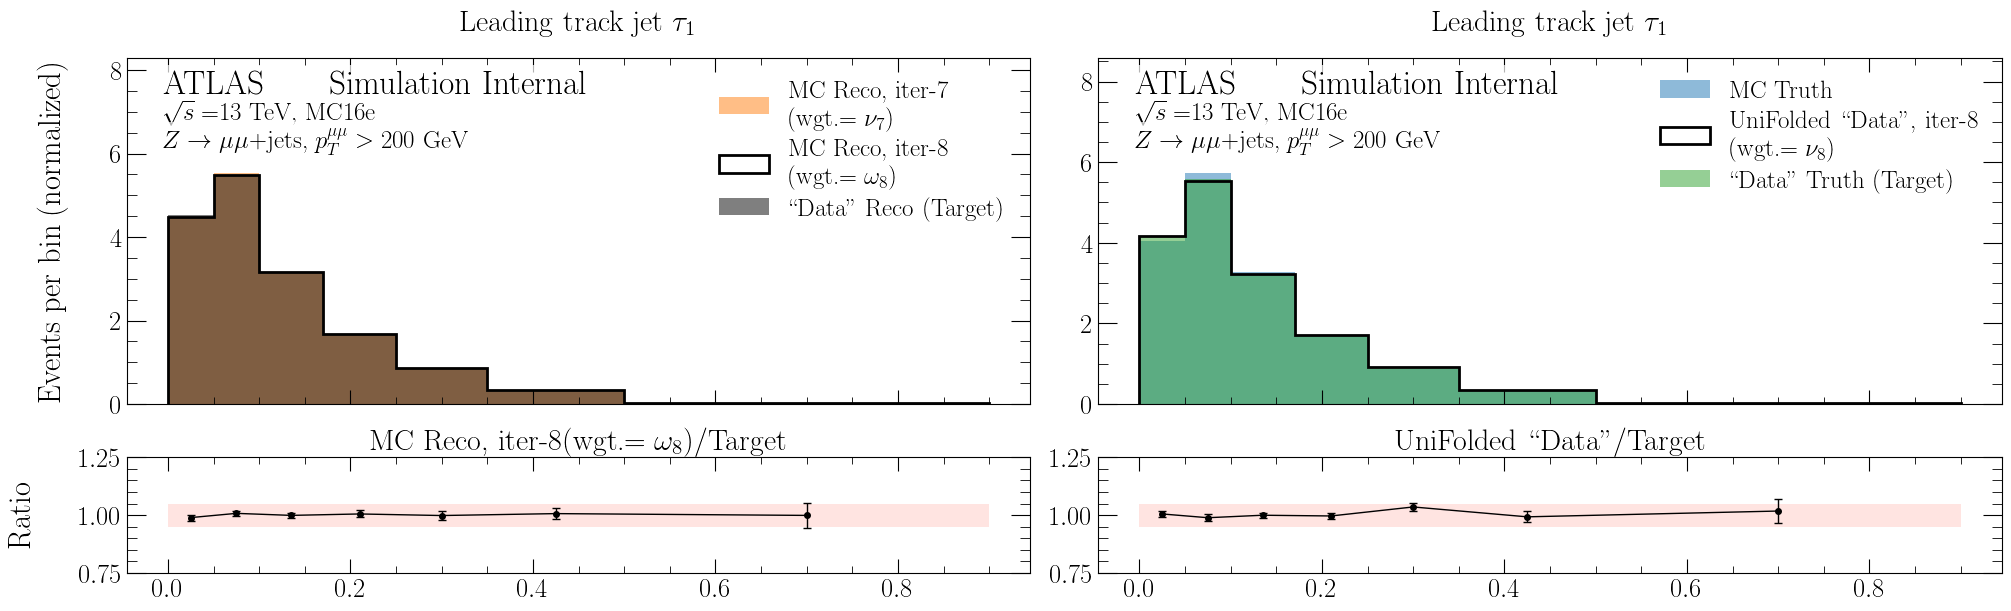
\includegraphics[width=0.95\textwidth]{figures/num_iterations_study/tau1_trackj1/iteration_study_30x10-Iteration08.png}}\\
\subfloat[Iteration 9]{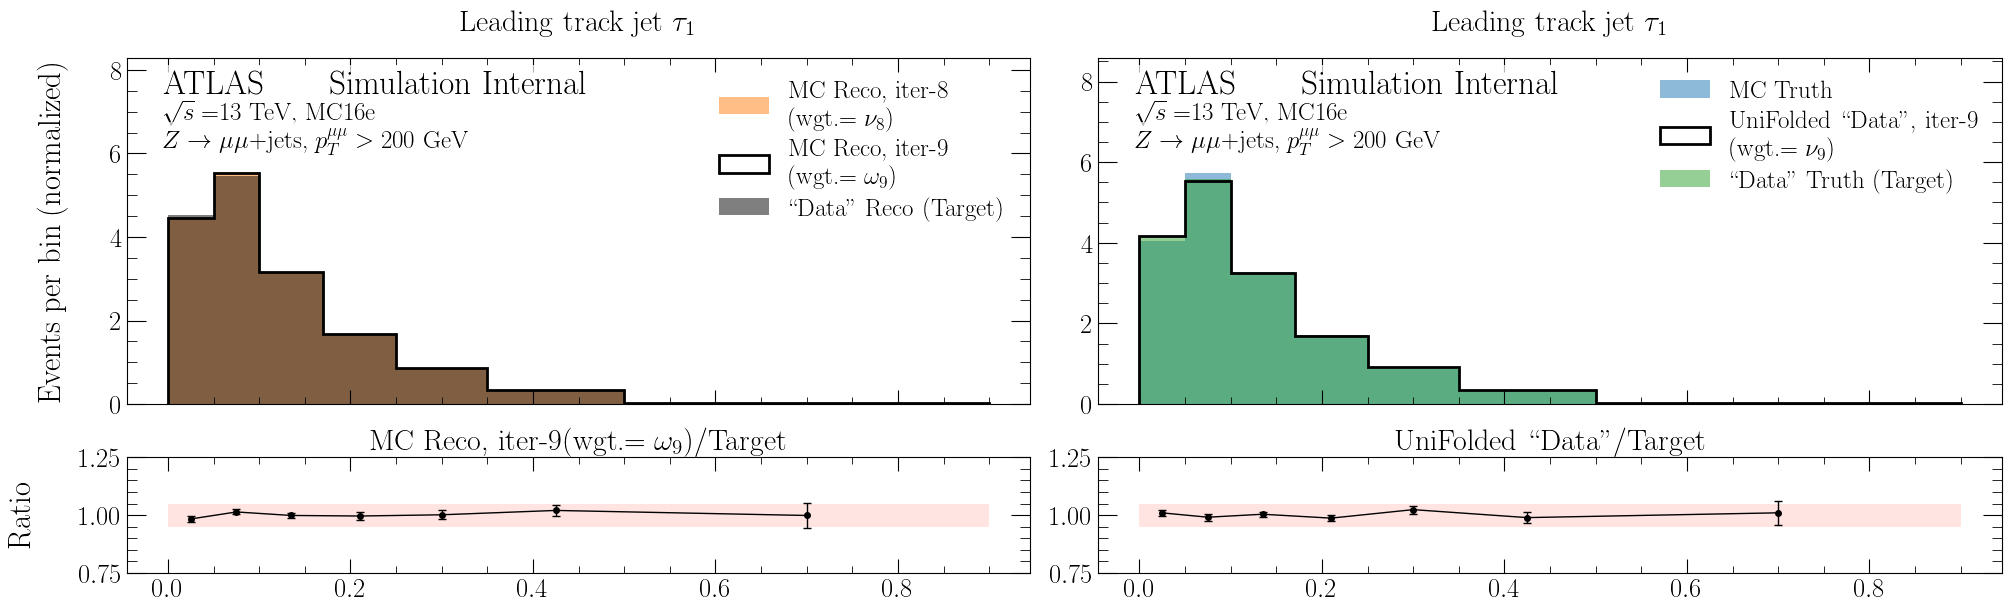
\includegraphics[width=0.95\textwidth]{figures/num_iterations_study/tau1_trackj1/iteration_study_30x10-Iteration09.png}}\\
\subfloat[Iteration 10]{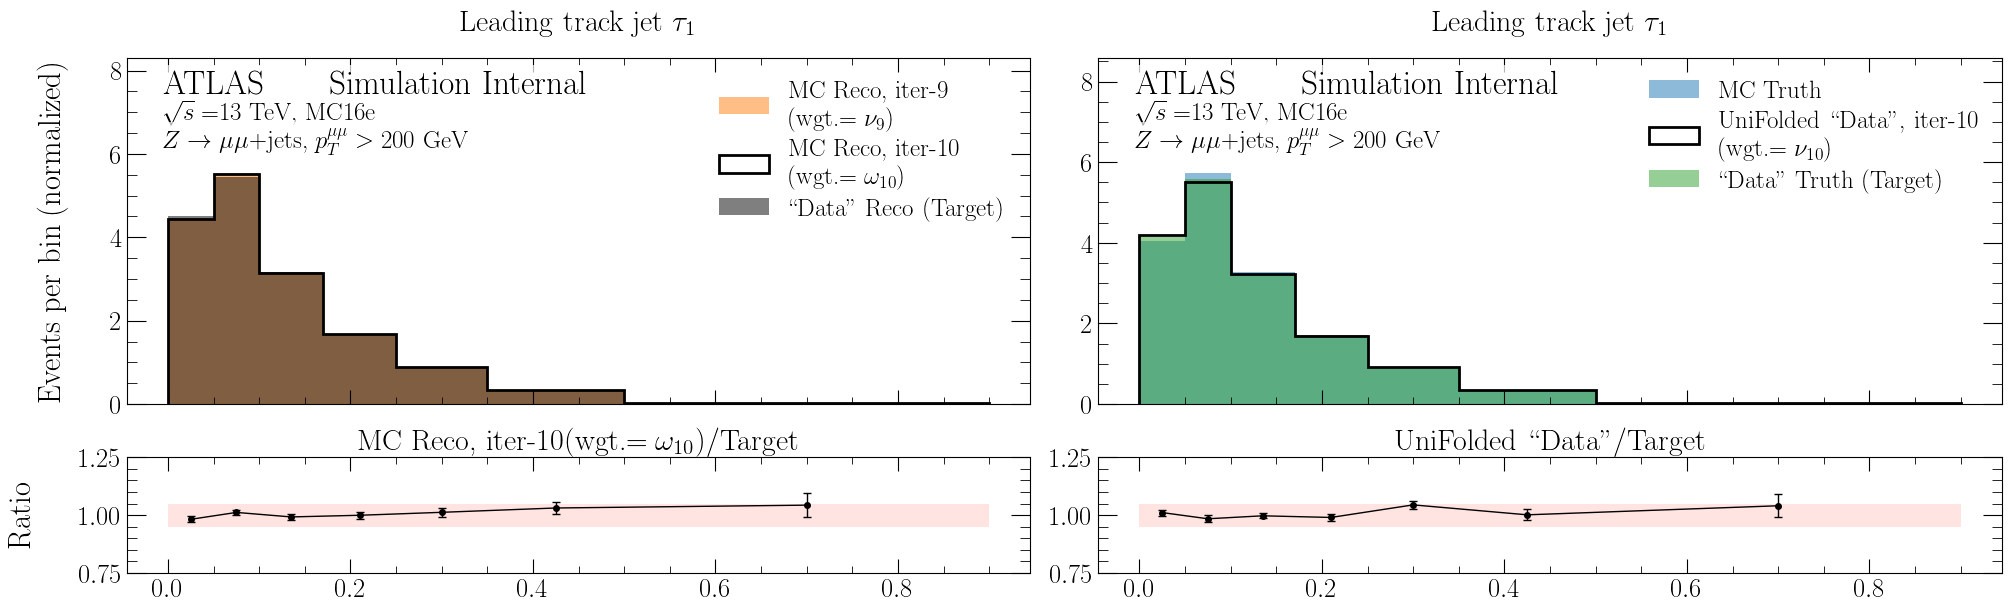
\includegraphics[width=0.95\textwidth]{figures/num_iterations_study/tau1_trackj1/iteration_study_30x10-Iteration10.png}}
\caption{\textbf{Leading jet $\tau_1$:} The unfolded histograms for UniFold in a single trial with Poisson bootstrapping applied. The ratio plots reveal that the bulk of the distribution quickly achieves good performance after about two iterations, but the tails of the distribution can sometimes benefit from additional iterations.}
\label{fig:num_iterations:tau1_ratios}
\end{figure}


\subsubsection{Performance as a function of iteration}
\begin{figure}[!htb]
\centering
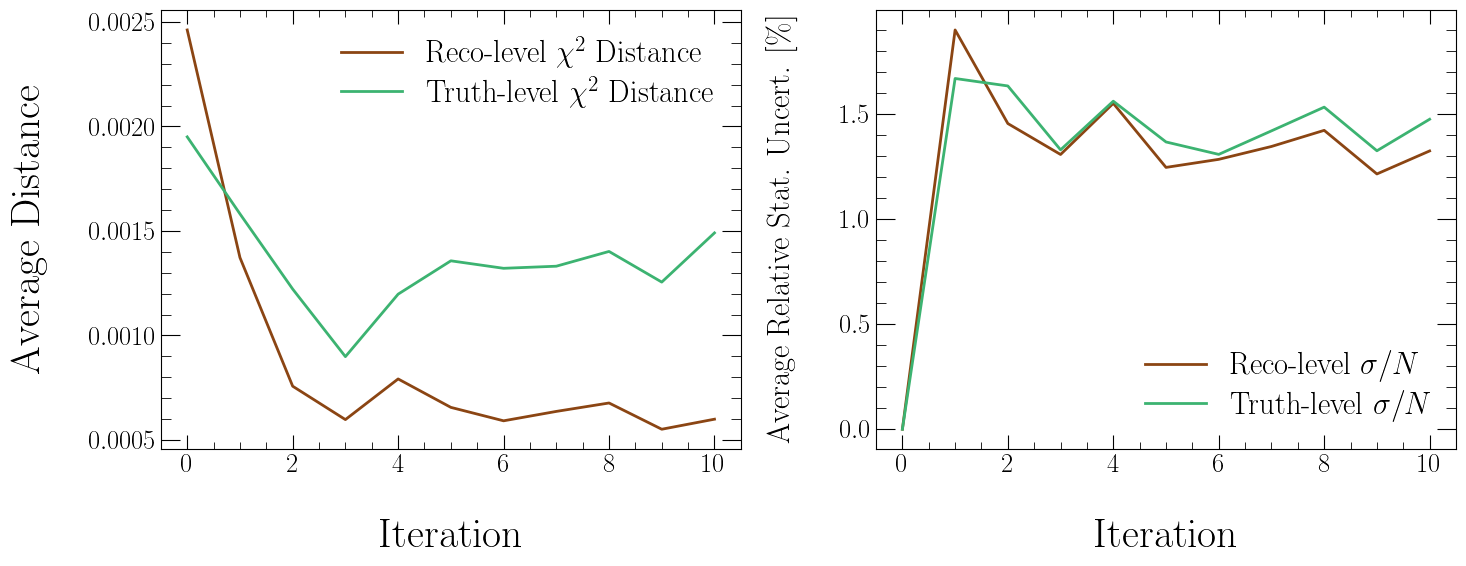
\includegraphics[width=0.95\textwidth]{figures/num_iterations_study/tau1_trackj1/iteration_study_30x10-distances-and-stat-uncert.png}\\
\caption{\textbf{Leading jet $\tau_1$:} On the left, average $\chi^2$ histogram distance per iteration, and on the right, average relative statistical uncertainty per iteration.}
\label{fig:num_iterations:tau1_distances_stat_uncert}
\end{figure}
\begin{figure}[!htb]
\centering
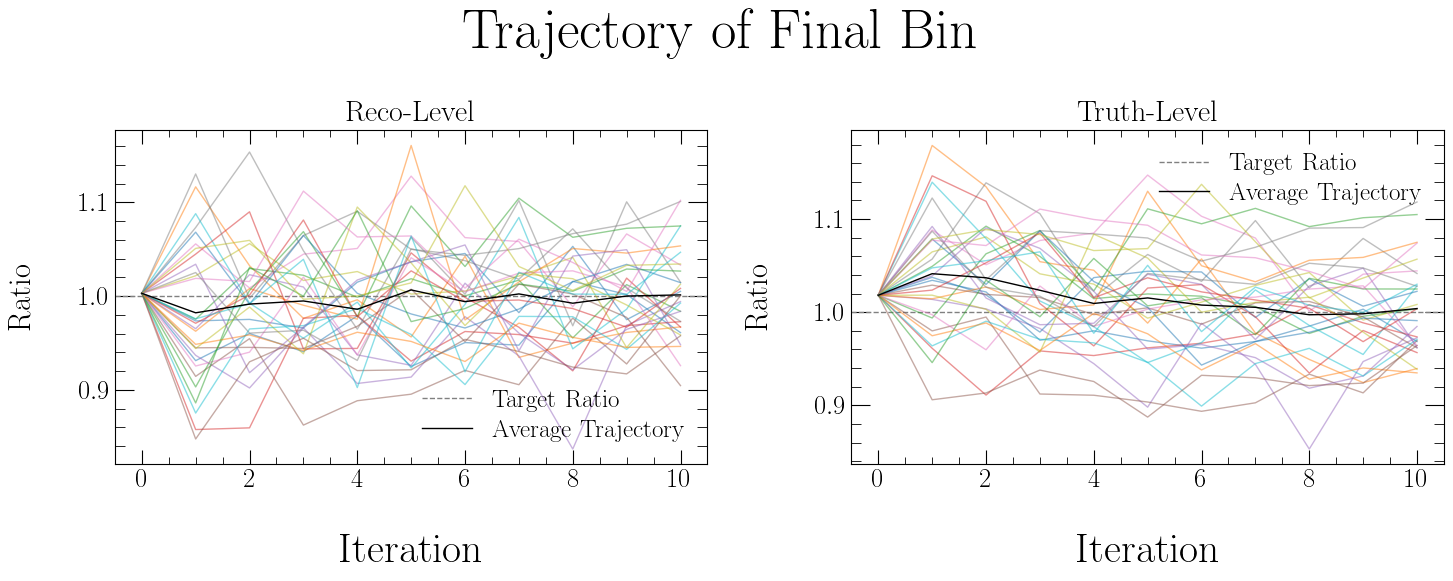
\includegraphics[width=0.95\textwidth]{figures/num_iterations_study/tau1_trackj1/iteration_study_30x10-final_bin.png}\\
\caption{\textbf{Leading jet $\tau_1$:} Trajectories of the final bin for each of the 30 bootstrapped independent trials as well as the average trajectory. The ratio is the unfolded histogram with respect to the target histogram.}
\label{fig:num_iterations:tau1_final_bin}
\end{figure}



